% Important: The shell-escape flag is required for the Minted package.
% Please compile this document with 'pdflatex -shell-escape main.tex'.
% If you are using another IDE, you may be able to specify this in the
% options or to provide an option like '% !TEX option = -shell-escape'
% in this file, depending on your builder. See the README.md for more.

% Don't put any content in here.
% Don't even include content files by using \input or \inlcude.
% Put your content into components/text.tex or include it there using \input.
% You probably want to modify the following files:
%   components/info.tex             contains the author, title etc.
%   components/settings.tex         contains the packages and settings.
%   components/commands.tex         contains helpful custom commands.
%   components/glossary.tex         contains an explanation of the used terms.
%   components/acknowledgements.tex contains the acknowledgements.
%   components/quote.tex            contains a quote.
%   components/abstract.tex         contains the abstract of the document.
%   components/text.tex             includes the actual content of the document.
%   components/outline.tex          contains the outline.
%   components/preface.tex          contains the preface.
%   chapters/                       contains the main text.
%   bibliography/literature.bib     contains the BibTeX entries.
%   images/                         contains all your content-related images.
%
% You probably don't need to change anything in the following files:
%   components/cover.tex            formats the front cover of the document.
%   components/titlepage.tex        formats the title page of the document.
%   components/disclaimer.tex       formats the disclaimer page.
%   styles/                         contains style elements (e.g. logos).
%   main.tex                        contains the top-level code structure.
%   README.md                       contains information about this template.

\documentclass[11pt,
a4paper,
index=totoc,
headsepline,
footsepline,
BCOR12mm,
oneside, %TODO verify with Dietrich
DIV13]{scrbook}

% KOMA scrbook options:
%  index=totoc: include an entry for the index in the table of contents.
%  headsepline: use horizontal line under heading.
%  footsepline: use horizontal line above footer.
%  BCOR: binding correction (e.g.: BCOR12mm)
%  DIV: Number of sheet sections (used for layout) (e.g.: DIV13)

% !TEX root = ../main.tex
% Set here the title, authors and other stuff to be used for the cover
% This file is used by MAIN.TEX

% set title, authors and stuff for the cover
\def\university{Technical University Munich}
\def\universityLogo{styles/tum_logo}
\def\program{Department of Informatics}
\def\programLogo{images/infologo}
\def\doctype{Bachelor's Thesis in Informatics}

\def\title{Combining Sentiment Analysis with Topic Modeling on Streamed Social Network Data}
\def\titlegerman{Kombination von Topic Modeling und Sentimentanalyse auf Streamed Social Media Daten}
\def\author{Claas Meiners}
\def\examinerOne{PD Dr.\ Georg Groh}
\def\assistantAdvisor{Dietrich Trautmann, MSc.}
\def\date{October 16th, 2017}

\def\keywords{{sentiment analysis}, {topic modeling}, {streaming}, {social media}}

% The following are used for the PDF metadata, by default the same as above.
\def\metaTitle{\title}
\def\metaAuthor{\author}
\def\metaSubject{\doctype\ -\ \university}
\def\metaKeywords{\keywords}

% text to appear in the footer
\def\footertext{}


% !TEX root = ../main.tex
% Included by MAIN.TEX

%--------------------------------------------------
% Fonts and page setup
%--------------------------------------------------

% Default font
\usepackage{palatino}

% Enable special PostScript fonts (optional)
% \usepackage{pifont}

% Manipulate the footer
\usepackage{scrpage2}
\usepackage{scrhack}
\pagestyle{scrheadings}
\ifoot[\footertext]{\footertext} % \footertext set in INFO.TEX

% Set the font for the section headings
\renewcommand{\sectfont}{\normalfont \bfseries}

% Conditional commands in LaTeX documents, used for the \clearemptydoublepage.
\usepackage{ifthen}

% Typeset text in multiple columns (optional)
% \usepackage{multicol}

% Rotation tools, including rotated full-page floats (optional)
\usepackage{rotating}


%--------------------------------------------------
% Document structure
%--------------------------------------------------

% Create glossaries and lists of acronyms
\usepackage[toc, xindy]{glossaries}

% Standard LaTeX package for creating indexes
\usepackage{makeidx}


%--------------------------------------------------
% Bibliography
%--------------------------------------------------

% Set the bibliography style (default: plain)
\bibliographystyle{plain}

% Special biblography package (nice to have)
% \usepackage{natbib}


%--------------------------------------------------
% Graphics and floats
%--------------------------------------------------

% Enhanced support for graphics (recommended)
\usepackage{graphicx}
% Path to the figures directory (default: {figures/})
% Multiple entries are allowed, e.g. {{figures1/}{figures2/}}.
\graphicspath{{figures/}}

% Improved interface for floating objects (optional)
\usepackage{float}

% To use the subfigures (optional)
\usepackage{subcaption}


%--------------------------------------------------
% Mathematics
%--------------------------------------------------

% AMS mathematical facilities for LaTeX (recommended)
\usepackage{amsmath}

% TeX fonts from the American Mathematical Society (recommended)
\usepackage{amsfonts}

% Some extra math symbols (optional)
% \usepackage{amssymb}

% Extended maths fonts for LaTeX (optional)
% \usepackage{yhmath}

% Provide math delimiters whose size can be computed automatically (optional)
% \usepackage{commath}


%--------------------------------------------------
% Source code and algorithms
%--------------------------------------------------

% Source code typesetting
% \usepackage{listings} % (optional - alternative)
\usepackage[newfloat]{minted} % (recommended)
% Set global Minted options
\setminted{linenos, autogobble, frame=lines, framesep=2mm}
% Inline C++ (optional)
\newcommand{\incpp}[1]{\mintinline{c++}{#1}}
\newenvironment{code}{\captionsetup{type=listing}}{}
\SetupFloatingEnvironment{listing}{name=Source Code}

% Typeset algorithms - pseudocode (optional)
% \usepackage{algorithmicx}
% \usepackage{algpseudocode}
% Normal arrow comments
% \algrenewcommand{\algorithmiccomment}[1]{\hfill$\rightarrow$ #1}


%--------------------------------------------------
% Tables
%--------------------------------------------------

% Tables (optional)
\usepackage{tabu}

% Add color to LaTeX tables (optional)
% \usepackage{colortbl}

% Create tabular cells spanning multiple rows (optional)
% \usepackage{multirow}


%--------------------------------------------------
% Color
%--------------------------------------------------

% Use colors
\usepackage[dvipsnames]{xcolor}

% You may find all the pre-defined colors in
% https://en.wikibooks.org/wiki/LaTeX/Colors#Predefined_colors

% Custom colors
\definecolor{Pantone300C}{HTML}{0065BD} % TUM primary blue
\definecolor{Pantone301}{HTML}{005293}  % TUM secondary light blue
\definecolor{Pantone540}{HTML}{003359}  % TUM secondary dark blue
\definecolor{DarkGray}{HTML}{333333}    % TUM secondary dark gray
\definecolor{MediumGray}{HTML}{808080}  % TUM secondary medium gray
\definecolor{LightGray}{HTML}{CCCCC6}   % TUM secondary light gray
\definecolor{Pantone7527}{HTML}{DAD7CB} % TUM accent gray
\definecolor{Pantone158}{HTML}{E37222}  % TUM accent orange
\definecolor{Pantone383}{HTML}{A2AD00}  % TUM accent green
\definecolor{Pantone283}{HTML}{98C6EA}  % TUM accent very light blue
\definecolor{Pantone542}{HTML}{64A0C8}  % TUM accent light blue

% Color for the hyperlinks (e.g. table of contents)
\def\colorLinks{Pantone300C}
% Color for the web links
\def\colorUrl{Pantone542}
% Color for the citations
\def\colorCitations{Pantone158}

%--------------------------------------------------
% PDF output
%--------------------------------------------------

% Pro­duce hy­per­text links in the doc­u­ment (recommended)
\usepackage{hyperref}

% Adjust the color of the links
\hypersetup{
  linkcolor=\colorLinks,%
  urlcolor=\colorUrl,%
  citecolor=\colorCitations
}

% Disable the coloring of the links when printing.
% Requires a compatible PDF reader.
\usepackage[ocgcolorlinks]{ocgx2}[2017/03/30]

% PDF Metadata
\hypersetup{
  pdftitle={\metaTitle},%
  pdfauthor={\metaAuthor},%
  pdfkeywords={\metaKeywords},%
  pdfsubject={\metaSubject}
}

% Create XMP Metadata (uses the values from hyperref)
\usepackage{hyperxmp}

% Make thumbnails (optional)
% \usepackage{thumbpdf}


%--------------------------------------------------
% Other settings
%--------------------------------------------------

% Define commands that appear not to eat spaces (optional)
\usepackage{xspace}


% !TEX root = ../main.tex
% Included by MAIN.TEX
% Please include your own cool commands here.
% Be only sure to comment it sufficiently so others can use it.

%-------------------------------------------------------------
%                      Own Commands
%-------------------------------------------------------------


%-------------------------------------------------------------
% math stuff -------------------------------------------------

% nice R, N, C
\newcommand{\nat}{\mathbb{N}}
\newcommand{\real}{\mathbb{R}}
\newcommand{\compl}{\mathbb{C}}

% norm
%\newcommand{\norm}[1]{\left\| #1 \right\|}

% un demi
\newcommand{\half}{\frac{1}{2}}

% parantheses
\newcommand{\parenth}[1]{ \left( #1 \right) }
\newcommand{\bracket}[1]{ \left[ #1 \right] }
\newcommand{\accolade}[1]{ \left\{ #1 \right\} }
%\newcommand{\angle}[1]{ \left\langle  #1 \right\rangle }

% partial derivative: %#1 function, #2 which variable
% simple / single line version
\newcommand{\pardevS}[2]{ \delta_{#1} f(#2) }

% fraction version
\newcommand{\pardevF}[2]{ \frac{\partial #1}{\partial #2} }

% render vectors: 3 and 4 dimensional
\newcommand{\veciii}[3]{\left[ \begin{array}[h]{c} #1 \\ #2 \\ #3	\end{array} \right]}
\newcommand{\veciv}[4]{\left[ \begin{array}[h]{c} #1 \\ #2 \\ #3 \\ #4	\end{array} \right]}

% render matrices: 3  dimensional (arguments in row first order)
\newcommand{\matiii}[9]{\left[ \begin{array}[h]{ccc} #1 & #2 & #3 \\ #4 & #5 & #6 \\ #7 & #8 & #9	\end{array} \right]}


%-------------------------------------------------------------
%-------------------------------------------------------------


%-------------------------------------------------------------
% some abreviations ------------------------------------------
\newcommand{\Reg}{$^{\textregistered}$}
\newcommand{\reg}{$^{\textregistered}$ }
\newcommand{\Tm}{\texttrademark}
\newcommand{\tm}{\texttrademark~}
\newcommand {\bsl} {$\backslash$}

%-------------------------------------------------------------
%-------------------------------------------------------------


%-------------------------------------------------------------
% formating --------------------------------------------------

% Theorem & Co environments and counters
\newtheorem{theorem}{Theorem}[chapter]
\newtheorem{lemma}[theorem]{Lemma}
\newtheorem{corollary}[theorem]{Corollary}
\newtheorem{remark}[theorem]{Remark}
\newtheorem{definition}[theorem]{Definition}
\newtheorem{equat}[theorem]{Equation}
\newtheorem{example}[theorem]{Example}
%\newtheorem{algorithm}[theorem]{Algorithm}

% inserting figures
\newcommand{\insertfigure}[4]{ % Filename, Caption, Label, Width percent of textwidth
	\begin{figure}[htbp]
		\begin{center}
			\includegraphics[width=#4\textwidth]{#1}
		\end{center}
		\vspace{-0.4cm}
		\caption{#2}
		\label{#3}
	\end{figure}
}

% referecing figures

\newcommand{\refFigure}[1]{ %label
	figure \ref{#1}
}
\newcommand{\refChapter}[1]{ %label
	chapter \ref{#1}
}

\newcommand{\refSection}[1]{ %label
	section \ref{#1}
}

\newcommand{\refParagraph}[1]{ %label
	paragraph \ref{#1}
}

\newcommand{\refEquation}[1]{ %label
	equation \ref{#1}
}

\newcommand{\refTable}[1]{ %label
	table \ref{#1}
}

\newcommand{\rigidTransform}[2]
{
	${}^{#2}\!\mathbf{H}_{#1}$
}

% comment that appears on the border - very practical !!!
\newcommand{\comment}[1]{\marginpar{\raggedright \noindent \footnotesize {\sl #1} }}

% page clearing
\newcommand{\clearemptydoublepage}{%
  \ifthenelse{\boolean{@twoside}}{\newpage{\pagestyle{empty}\cleardoublepage}}%
  {\clearpage}}

%-------------------------------------------------------------
%-------------------------------------------------------------

\newcommand{\etAl}{\emph{et al.}\mbox{ }}


% !TEX root = ../main.tex
\newglossaryentry{computer}
{
  name=computer,
  description={is a programmable machine that receives input,
               stores and manipulates data, and provides
               output in a useful format}
}

\newglossaryentry{poc}
{
  name={proof of concept},
  description={}
  }
\newglossaryentry{ui}
{
  name={user interface},
  description={}
  }
\newglossaryentry{ai}
{
  name={arithmetic intensity},
  description={a measure of floating-point operations (FLOPs)
              \hyphenation{per-formed} performed by a \hyphenation{gi-ven} given code or code section relative
              to the amount of memory accesses (Bytes) that are required
               to support those operations\cite{AI}}
  }

\newglossaryentry{speed-up}
{
  name={speed-up},
  description={the factor of temporal acceleration a program
  exhibits when additional computational resources are dedicated to it's execution.}
}

\newglossaryentry{directive pragmas}
{
  name={directive pragma},
  description={a computer programming language construct that specifies how a compiler
  should process input data} % sourced from wikipedia
}


\newglossaryentry{rc}{%SOURCE: wikipedia
name={race condition},
description={A race condition or race hazard is the behavior of an electronic,
 software, or other system where the output is dependent on the sequence or
 timing of other uncontrollable events. It becomes a bug when events do not
 happen in the order the programmer intended. The term originates with the idea
 of two signals racing each other to influence the output first.}
}
\newglossaryentry{dd}{
name={data dependencies},
description={}
}
\newglossaryentry{sisd}{
name={single instruction single data},
description={}
}
\newglossaryentry{simt}{
name={single instruction multiple threads},
description={}
}

\newglossaryentry{simd}{
name={single instruction multiple data},
description={}
}
\newglossaryentry{gp}{%SOURCE: wikipedia
name={Gaussian Plane},
description={The two dimensional plane of complex numbers.}
}
\newglossaryentry{CURAND}{
name={CURAND},
description={
The CURAND library provides facilities that focus on the simple and efficient
generation of high-quality pseudorandom and quasirandom numbers.\cite{cuRAND}
}
}

\newacronym[longplural={partial differential equations}]{PDE}{PDE}{partial differential equations}
\newacronym{mpi}{MPI}{Message Passing Interface}

\newacronym[longplural={Random Walks on Spheres}]{RWoS}{RWoS}{Random Walk on Spheres}

\newacronym[longplural={graphical processing units}]{GPU}{GPU}{graphical processing unit}

\newacronym[longplural={central processing units}]{CPU}{CPU}{central processing unit}
\newacronym{hpc}{HPC}{high performance computing}

\newacronym[longplural={arithmetic logic units}]{ALU}{ALU}{arithmetic logic unit}

\newacronym[longplural={streaming multi-processors}]{SM}{SM}{streaming multi-processor}

\newacronym[longplural={boundary value problems}]{BVP}{BVP}{boundary value problem}
\newacronym[longplural={general purpose graphical processing units}]{GPGPU}{GPGPU}{general purpose graphical processing units}
\newacronym{CUDA}{CUDA}{compute unified device architecture}
\newacronym{RAM}{RAM}{random access memory}
\newacronym{SRAM}{SRAM}{static random access memory}
\newacronym{DRAM}{DRAM}{dynamic random access memory}
\newacronym{I/O}{I/O}{input/output}
\newacronym{PTX}{PTX}{Parallel Thread eXecution}
\newacronym{jit}{JIT}{just in time}


\makeglossary

\begin{document}

    \frontmatter

    % !TEX root = ../main.tex
% The front cover.
% Included by MAIN.TEX

%--------------------------------------------------
% The Front Cover
%--------------------------------------------------

% correct BCOR - undo at the end !!!
\def\bcorcor{0.15cm}
\addtolength{\hoffset}{\bcorcor}

\thispagestyle{empty}

\vspace{4cm}
\begin{center}
	\includegraphics[width=4cm]{\universityLogo}\\
	\vspace{5mm}
	\huge \program \\
	\vspace{0.5cm}
	\large \university
\end{center}

\vspace{20mm}
\begin{center}
	{\Large \doctype}\\
	\vspace{20mm}
	{\huge \textbf \title}\\
	\vspace{15mm}
	{\LARGE  \author}\\
	\vspace{\fill}
	\includegraphics[width=4cm]{\programLogo}
\end{center}


    \clearemptydoublepage

    % !TEX root = ../main.tex
% The titlepage.
% Included by MAIN.TEX


%--------------------------------------------------
% The title page
%--------------------------------------------------

% correct BCOR - undo at the end !!!
\def\bcorcor{0.15cm}
\addtolength{\hoffset}{\bcorcor}

\thispagestyle{empty}

\vspace{4cm}
\begin{center}
    \includegraphics[width=4cm]{\universityLogo}\\
    \vspace{5mm}
    \huge \program \\
    \vspace{0.5cm}
    \large \university
\end{center}

\vspace{10mm}
\begin{center}
    {\Large \doctype}\\
    \vspace{10mm}
    {\LARGE \title}\\
    \vspace{10mm}
    {\LARGE \titlegerman}\\
    \vspace{10mm}

    \begin{tabular}{ll}
      \Large Author:                        & \Large \author \\[2mm]
      \Large 1\textsuperscript{st} examiner:& \Large \examinerOne\\[2mm]
      %\Large 2\textsuperscript{nd} examiner:& \Large \examinerTwo \\[2mm]
      \Large Assistant advisor:             & \Large \assistantAdvisor \\[2mm]
      \Large Submission Date:               & \Large \date
    \end{tabular}

    \vspace{\fill}
    \includegraphics[width=4cm]{\programLogo}
\end{center}

% undo BCOR correction
\addtolength{\hoffset}{\bcorcor}


    % !TEX root = ../main.tex
\clearemptydoublepage

\thispagestyle{empty}
\vspace*{0.8\textheight}
\noindent
I hereby declare that this thesis is entirely the result of my own work except where otherwise indicated. I have only used the resources given in the list of references.

\vspace{15mm}
\noindent
\date \hspace{5cm} \author
\newpage


    % !TEX root = ../main.tex
\clearemptydoublepage
\phantomsection
\addcontentsline{toc}{chapter}{Acknowledgements}

\vspace*{2cm}

\begin{center}
{\Large \textbf Acknowledgments}
\end{center}

\vspace{1cm}

\begin{center}
Professors and tutors, friends and family TODO
\end{center}


    % !TEX root = ../main.tex
% The abstract.
% Included by MAIN.TEX

\clearemptydoublepage
\phantomsection
\addcontentsline{toc}{chapter}{Abstract}

\vspace*{2cm}
\begin{center}
{\Large \textbf Abstract}
\end{center}
\vspace{1cm}

I'll write the abstract at the end, it'll about fill two thirds of the remainder of this page.
TODO




    \tableofcontents

    \mainmatter

    % !TEX root = ../main.tex
% Included by MAIN.TEX
% Put your content in here or include it by using \input (\include won't work)

\addtolength{\evensidemargin}{-12mm}

% ---------------------------------------------------------------------------
%
%Introduction and Background Theory
%
% ---------------------------------------------------------------------------
\part[Introduction]{Introduction and Background Theory}
\label{part:introAndBackgroundTheory}
% !TEX root = ../main.tex

\chapter{Motivation}
\label{ch:motivation}

% A definition of social media in general
Social media is defined as an application with a set of characterizing features \cite{Ellison2008}:
\begin{enumerate}
    \item
    Creating a profile containing personal information such as location or age, as well as pictures and optionally other kinds of multimedia content
    \item
    Building a list of connected profiles facilitating relationships such as friendship
    \item
    Seeing and traversing lists of connections from your own and other profiles
\end{enumerate}

% Some examples of social media, including twitter, which I focus on in this thesis

The first application that can be classified as social media according to these characterisitics
was the web-based service SixDegrees.com, launched in 1997 \cite{Ellison2008}.
A timeline of this and other selected social media application launches can be seen in \ref{fig:timeline}.

\begin{figure}
    \caption{A timeline of selected social media launches.}
    \label{fig:timeline}
    \begin{chronology}[5]{1997}{2017}{\linewidth}
        \event{1997}{\small{SixDegrees.com}}
        %\event{1999}{LiveJournal}
        %\event{1999}{AsianAvenue}
        %\event{1999}{BlackPlanet}
        %\event{2000}{MiGente}
        %\event{2001}{CyWorld}
        %\event{2001}{Ryze}
        %\event{2001}{Fotolog}
        \event{\decimaldate{22}{3}{2002}}{\small{Friendster}}
        %\event{\decimaldate{5}{5}{2003}}{\small{LinkedIn}}
        \event{\decimaldate{1}{8}{2003}}{\small{MySpace}}
        %\event{2003}{\small{Xing}}
        \event{\decimaldate{4}{2}{2004}}{\small{Facebook}}
        %\event{\decimaldate{10}{2}{2004}}{\small{Flickr}}
        \event{\decimaldate{15}{7}{2006}}{\small{Twitter}}
        \event{\decimaldate{6}{10}{2010}}{\small{Instagram}}
        \event{\decimaldate{28}{6}{2011}}{\small{Google Plus}}
        \event{\decimaldate{24}{1}{2013}}{\small{Vine}}
    \end{chronology}
\end{figure}

Apart from the 3 main characterizing features, social media applications vary greatly in functionality.
Most offer messaging and blogging capabilities, while some even allow for more specific use cases like live video-streaming \cite{Ellison2008}.

\begin{table}
    \caption{A comparison of social media applications}
    \label{tab:comparison}
    \resizebox{\textwidth}{!}{%
    \begin{tabular}{lllll} %
        \toprule
        & & \multicolumn{2}{c}{Main Relationship Type} & \\
        \cmidrule{3-4}
        Name
        & Main Content Types
        & Name
        & Characteristics
        & Platforms
        \\
        \midrule
        Facebook
        & Text, images, videos, live-stream
        & Friendship
        & Two-sided, balanced
        & Web and App
        \\
        \midrule
        Twitter
        & Text (limited to 140 characters)
        & Following
        & One-sided, unbalanced
        & Web and App
        \\
        \midrule
        Instagram
        & Images
        & Following
        & One-sided, unbalanced
        & Web and App
        \\
        \midrule
        Google Plus
        & Text, images, videos
        & Friendship
        & Two-sided, balanced
        & Web and App
        \\
        \midrule
        Vine
        & Videos
        & Following
        & One-sided, unbalanced
        & App
        \\
        \bottomrule
    \end{tabular}}
    %TODO figure footnote: unbalanced* -> few accounts with most of the followers
    %TODO google plus: being in the same circle
\end{table}

As seen in~\ref{tab:comparison}, not all social media applications are solely web-based services.
Some, such as Vine, do not even offer a web-based interface anymore.
Also, only few of the social media applications analyzed offer networking capabilities in the sense of two-sided relationship initiation,
meaning there is no focus on creating relationships online that are then transferred into the real world.
For these reasons, this thesis refrains form using the term social networking site (SNS), as commonly used in previous works \cite{Ellison2008},
and instead uses the term social media application.
\par

% Social media is big and growing
The first indication of the growing importance and influence of social media can be found by looking at the growth numbers:
Facebook, for example, has more than 1 billion users to date, and Twitter's userbase grew by 1,382\% between February 2008 and February 2009 \cite{mcgiboney2009twitter} alone.
\par

% Social media influences elections...
It is estimated that during the 2016 U.S. election, american adults read and remembered on the order of one to several so called fake news;
untruths portrayed as news favoring a specific candidate.
Although no assessment can be made as to whether the influence of fake news was pivotal to the election,
evidence can be found supporting the claim that exposure to fake news influences a voters sentiment \cite{Allcott2017}.
\par
% ...and companies
Furthermore, social media applications changed the way organisations, communities and individuals communicate.
Customers expect companies to listen to and engage with them on these channels - and past approaches to customer care are ill-suited for this new environment \cite{Kietzmann2011}.
\par
Most of the recent growth in social media usage happened in a important target demographic for companies -
65\% of american adults were using social media in 2015, almost 10 times more than in 2005, when only 7\% did \ref{Perrin2015}.
\par
Similar developments can be observed in the amount of goods and services sold via the internet:
The share of e-commerce in the total U.S. retail sales grew from 4.2\% in the first quarter of 2010 to more than double that, 8.5\%, by the second quarter of 2017, a mere 7 years later \cite{statistaECommerceGrowth}.
This growth will continue and the change from traditional commerce to e-commerce
will further influence the way customers interact with companies.
\par
The growing importance and influence of social media for companies and individuals,
paired with the potential for misuse as demonstrated during the 2016 election,
necessitates improved real-time monitoring capabilities for the affected stakeholders.
\par
From an organizational standpoint, complaints, comments, questions and suggestions by the customer are not only unstructured,
but also "designed by the customer", meaning that the organization has little influence on the way customers choose to communicate with them.
Since many customers are already familiar with social media, it often becomes the medium of choice for communicating with companies.
However, no standardized rules exist for these kind of transactions, making reporting, analysis and knowledge management on the companies side difficult \cite{Culnan2015}.
\par
This thesis aims to explore and implement means of monitoring topics of interaction on social media in real-time,
and combine this analysis with the associated sentiment, to provide informative insights for these stakeholders.

% First justification why we are using twitter TODO put this somewhere else
Twitter's main content type as shown in~\ref{tab:comparison} consists of small, simple text entries, called tweets, with a maximum length of 140 characters,
which makes it popular among researchers, and a good fit
% !TEX root = ../main.tex

\chapter{Background Theory}

\label{ch:backgroundTheory}


%Social media is not used to its full potential by e.g. companies
Social media applications offer great opportunity for companies,
and while they are widely adopted and used,
companies struggle to achieve measurable business success with their social media work \cite{Culnan2015}.
\par
% There is reason to believe companies would benefit from being able to analyze what their customers talk about (topics) and how they feel about these topics (sentiment by topic)
This thesis theorizes that monitoring what users talk about,
and how they feel about what they talk about,
will enable stakeholders to get a more quantifiable and structured understanding of their target group.
\par
Culnan et al. \cite{Culnan2015} % TODO how to cite this better?
argue that identifying value metric is an element of effective social media implementation for companies.
This thesis theorizes that the topics users talk about, the sentiment there interactions have and the combination of these are such metrics.
\par
Furthermore, they argue that absorptive capacity (message and interaction processing) is one of the three main elements of social media implementation for companies.
This thesis theorizes that companies benefit from topic modeling, sentiment analysis and the combination of those being part of this processing.
\par
% What it could be used for, example use case
Not only could this real-time analysis be used to monitor consumer sentiment,
it could also be used to react to changes in sentiment among users in real-time to detect, prevent and counteract
drastic mood shifts (sometimes called shitstorms).
People responsible for managing social-media accounts with big influence may be exposed to and fear these kinds of online communication-crisis,
and being tasked with managing such an event poses great difficulty \cite{Salzborn2015}.
\par
% Using it as a feedback cycle for A/B testing.
Another benefit of monitoring the sentiment regarding a topic in real-time is that it could used for product development,
to compare different iterations of a product.
It could also be useful to rapidly iterate social media marketing strategies.
%TODO add some graphic here, and maybe divide into sub-chapters
%TODO also a double pagebreak between chapters is very unnecessary.
% !TEX root = ../main.tex
\chapter{Goals}
\label{ch:goals}

The goal of this thesis is to develop a solution that enables its users to monitor,
research and understand what Twitter users talk about and how they feel about it in real time,
visualizing and quantifying their activity on Twitter.
\\
A set of technologies appropriate for this application will be decided on and explained.
A quantitative comparison of methods used for sentiment analysis and topic modeling will be made,
exploring previous approaches and the special use case provided by Twitter.
The best method for this use case will then be determined.
\\
That way, this thesis will provide a way to analyze sentiment of statuses and model their topics,
as well as the combination of those.
\\
The final solution will provide a way to create a stream of statuses, analyzed in real time as they are posted on Twitter,
which can be filtered according to the users preferences to analyze only the activity most relevant to them.
\\
Most importantly, this solution will enable people not sufficiently familiar with technologies required to
implement such a real-time analysis application themselves to nevertheless research the topics and sentiment of real-time,
streamed social network data.
\\
The application will be  of a modular design, so that it can easily be expanded with different forms of analysis,
without requiring a full understanding of all the underlying technologies.

%
%% ---------------------------------------------------------------------------
%%
%% Thesis content: What did you do?
%%
%%% ---------------------------------------------------------------------------
\part[Body]{what was done for the tesis}
\label{part:body}
% !TEX root = ../main.tex

\chapter{Technologies used}

\label{ch:technologiesUsed}

I explain all the technologies used (excluding the dashboard) here, so that I can give code examples and talk about implementation
while introducing the theory for sentiment analysis and topic modeling, for the reader to be able to make the connection easier.

\textbf{Since it has great influence in the general structur: Do you think this is a good idea?}

The Libraries used for each of the algorithms will be explained in their respective chapters;
I only talk about technologes/design patterns etc that are used across all of them

NLTK is only really used in sentiment analysis, but since its such a prominent library, I'll do a general introduction here.
Is that okay, even though I don't introduce gensim here (since gensim is purpose-build for Topic Modeling)

Using the DS cookie cutter, except the streaming folder is one under source because it is used by data to collect training data and by visualization for the dashboard.
Generally a modular approach that can be easily expanded with further analysis/monitoring beyond the LDA/Sentiment Analysis with Naive Bayes combination has been build.

\begin{itemize}
    \item
    Spark offers some good data analysis functions (maybe show wordcount code here)
    \item
    Comparing the DataFrame-based and of the RDD-based API of Spark
    \item
    But Spark's real strength lies in the fact any library can be used on the execution node, which is why I use other libraries quite liberally for the best workflow (See chapters \ref{sentimentanalysis} and \ref{ch:topicModeling})
    \item
    The Factory pattern was used often because of how python handles scopes
    \item
    Why it makes sense and what is transmitted to the exec nodes in the end
    \item
    First using a queueStream, but it doesn\’t work in the python API, switched to starting a Kafka stream (Kafka just has to be running somewhere, on connect the stream is connected to the Kafka broker and the sparkjob is immediately submitted with the session id as a parameter)


\end{itemize}

\section{Architecture}
\label{sec:architecture}

Using the architecture from Book with a graphic cotaining ...

About 2 pages introducing the technologies.

\pagebreak[2]
% !TEX root = ../main.tex
\chapter{Twitter}
\label{ch:twitter}

\section{Introduction to Twitter}
\label{sec:twitter}

Twitter is a form of so-called microblogging, which is defined as a form of blogging with small-sized pieces of content,
usually text up to a character-count of 200, which, in the case of Twitter, are called Tweets or statuses
(where this thesis will stick to the latter since it is the predominant terminology used in the official documentation~\cite{twitterDocs}).
This enables light-weight, mobile and easy sharing of opinions, status and activities~\cite{Finin2007},
which proved popular among users and lead to rapid adoption and growth~\cite{mcgiboney2009twitter}.
\par
As shown in~\autoref{tab:comparison}, the relationships of following users and being followed by users on Twitter is unreciprocated,
which means it requires no active accepting of followers.\\
This leads to only 22.1\% of users who are being followed by someone, also being followed back by that someone~\cite{Kwak2010}.
Although Twitter offers the option to protect ones account, which means followers need to be accepted,
and users can be blocked, thereby denying them seeing ones content, these options are only used in rare cases,
making the form of relationships they represent the exception~\cite{Kwak2010}.\\
The relationship between different kinds of entities present on Twitter can be seen in~\autoref{fig:twitter}
\par

% include diagram
\begin{figure}
    \centering
    \caption{Simplified diagram of Twitter entity relations.}
    \label{fig:twitter}
    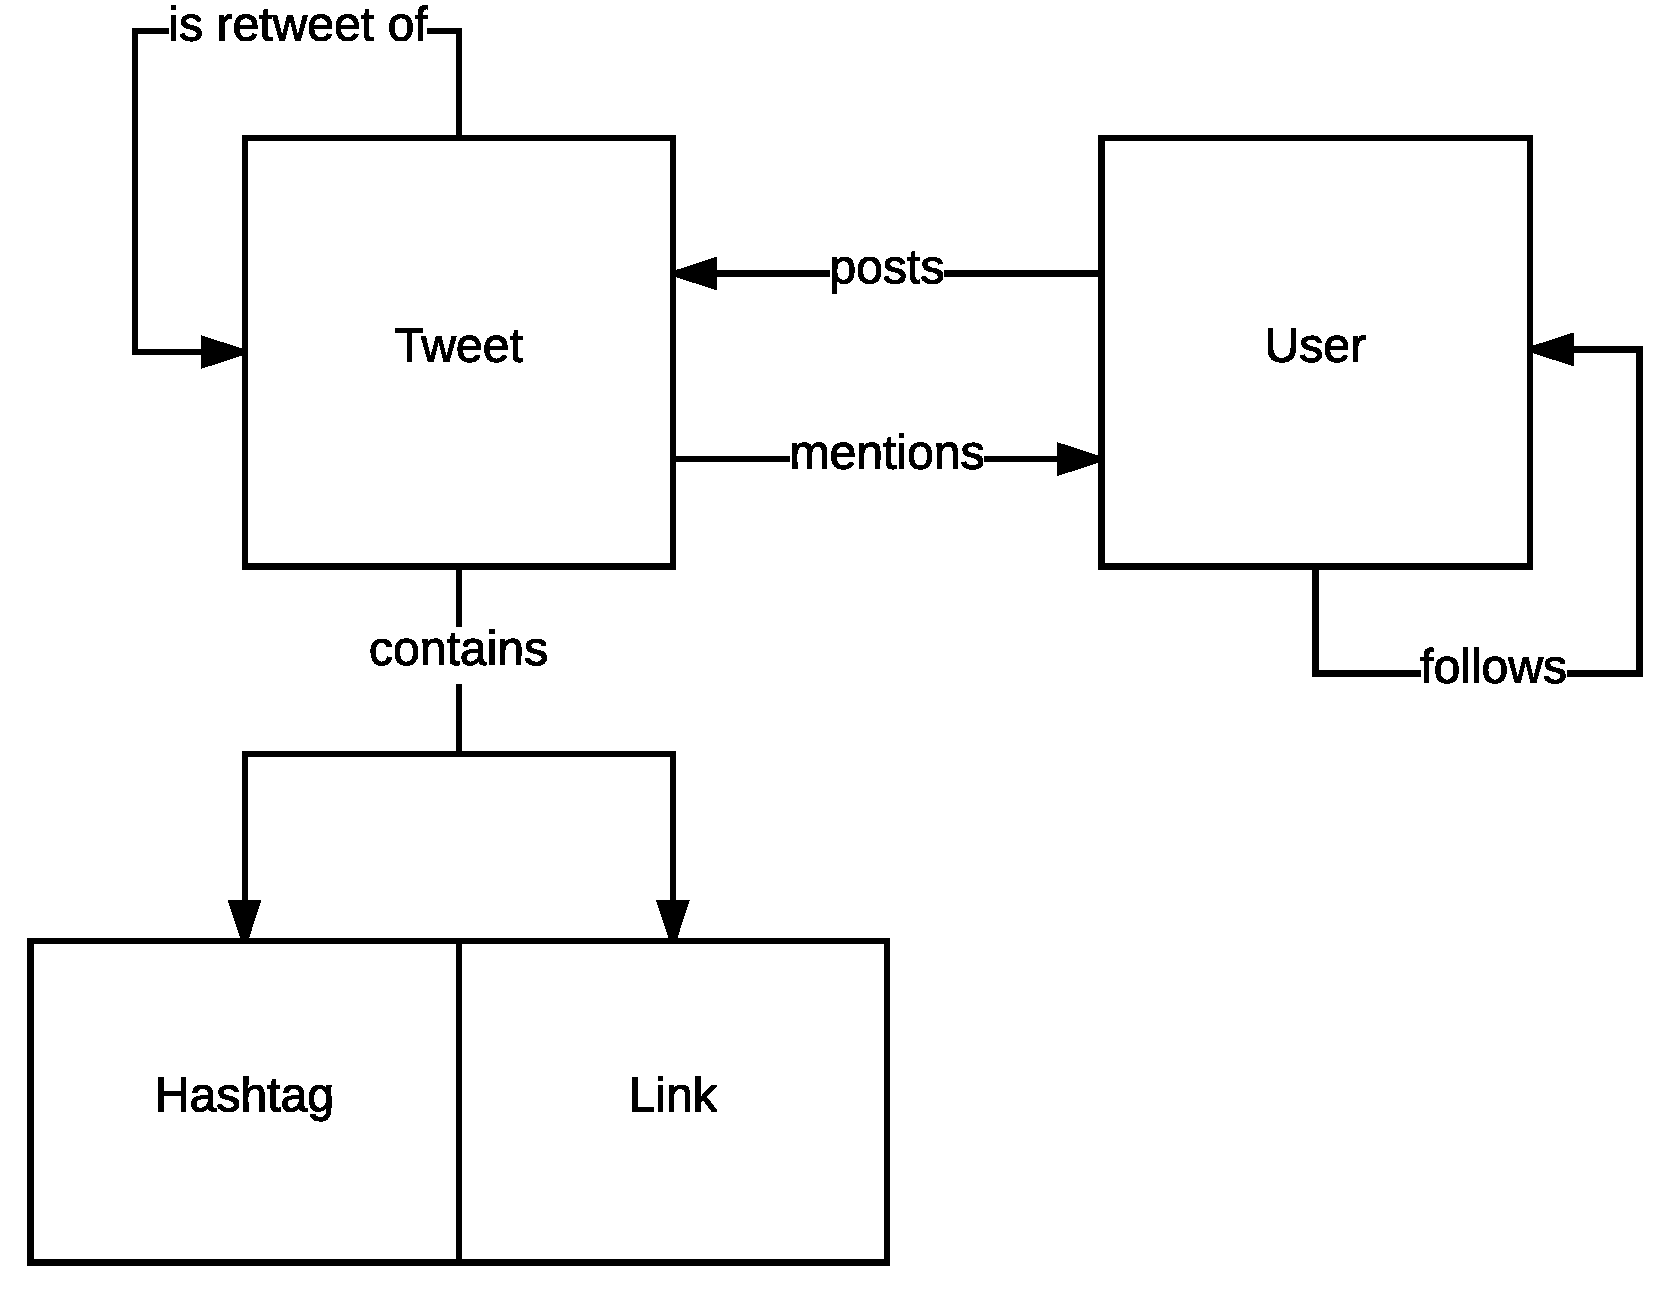
\includegraphics[width=10cm]{../figures/twitter_er.pdf}
\end{figure}

\par
This thesis will focus on analyzing statuses in real time.
Statuses on Twitter can not only contain text, but also rich media like images, gifs, or videos, as well as surveys.
The text itself can also contain links, mention other users by containing \texttt{@<user\_name>},
and contain any number of the infamous hashtag (\texttt{\#hashtag}), used to label a status, all while being limited to 140 characters.
A status can also be a so-called retweet of another status, adding to its content and exposing the other status to the retweeting users' followers.
Research shows that statuses are mostly retweeted shortly after they are published, and often lead to chains of retweets,
which not only spreads information fast, but also diffuses it~\cite{Kwak2010}.\\
\par
For the purpose of this thesis we will only focus on the text of a status and do not assign any special meaning to links,
mentions, hashtags or whether a status is a retweet.\\

\section{The Twitter API}
\label{sec:theApi}

Twitter is offering an API (\textbf{A}pplication \textbf{P}rogramming \textbf{I}nterface),
through which developers and researchers can access machine-readable data,
including the entities shown in~\autoref{fig:twitter}, from the platform.
This API transmits data encoded in JSON, and follows the REST-paradigm.
A Python-library called Tweepy, which contains utility functions for interaction with the Twitter API, was used where adequate~\cite{tweepyDocs}.

\subsection{JSON}
\label{subsec:json}

JSON (\textbf{J}ava\textbf{S}cript \textbf{O}bject \textbf{N}otation) is a data format originally conceptualized by ECMA international
for the programming language Javascript.
It was designed to be light-weight, human-readable yet easy for machines to generate and parse.
Due to this, and the fact that it uses conventions familiar to developers of C-like languages,
it has since become a widespread data-interchange format with libraries for parsing and generation in many languages~\cite{jsonDocs}.
A small example for an object in this format can be seen in~\autoref{code:json}.


%{
%    "apple": {
%        "calories": 123,
%        "contains_allergens": false
%        "types": ["Braeburh", "Cortland"]
%        "grows_on": "tree"
%    },
%    "hazelnut": {
%        "calories": 12,
%        "contains_allergens": true
%        "grows_on": "bush"
%    },
%}

\begin{figure}
    \caption{A shortened JSON representation of a fictional Twitter status}
    \label{code:json}
    % @formatter:off
    \begin{minted}{json}
    {
        "created_at" : "Fri Jan 20 20:04:05 +0000 2017",
        "id" : "123",
        "text" : "@other_user Hello!",
        "entities" : {
                "hashtags" : [],
                "symbols" : [],
                "user_mentions" : [{
                    "screen_name" : "other_user",
                    "name" : "Other User"}],
                "urls" : [] },
        "user" : {
            "name" : "User",
            "screen_name" : "user"
        }
    }
    \end{minted}
    % @formatter:on
\end{figure}

\subsection{REST}
\label{subsec:rest}

The Twitter API follows the REST (\textbf{RE}presentational \textbf{S}tate \textbf{T}ransfer) paradigm.
The REST-paradigm defines a set of architectural rules to ensure interoperability of distributed systems,
like clients and servers on the internet.
To achieve that, among other things,
it defines a set of methods that specify different kinds of operations that can be performed on data~\cite{Jakl2008}.
The most prevalent methods mentioned in the RFC are listed below~\cite{RFC2616}.

\begin{enumerate}
    \item
    \texttt{GET} - retrieves data identified by the URI (idempotent)
    \item
    \texttt{POST} - request to create a new entity, with the type specified by the URI
    \item
    \texttt{PUT} - request to create an entity identified by the URL, or update it if it exists (idempotent)
    \item
    \texttt{DELETE} - request to delete an entity identified by the URL (idempotent)
\end{enumerate}

There are more methods specified by the RFC~\cite{RFC2616} that will not be used in this thesis.
\par
The resources (also called API endpoints) offered by the Twitter REST-API are rate-limited,
which means any one application or Twitter-user using the API can make a limited number of requests to the API
per 15-minute time window.
Every request send to the API needs to be authenticated,
either as a Twitter user or as an application that can be registered in Twitter's developer console.
There are some resources which can only be accessed when a specific Twitter user authenticates
with the API, because they are user-specific, like publishing a status~\cite{twitterDocs}.
Some examples can be seen in ~\autoref{tab:twitter_endpoints}.

\begin{table}
    \caption{A selection of resources offered by the Twitter REST API~\cite{twitterDocs}}
    \label{tab:twitter_endpoints}
    \resizebox{\textwidth}{!}{
    \begin{tabular}{lllll} %
        \toprule
        & & \multicolumn{2}{c}{Authentication} & \\
        \cmidrule{3-4}
        Method
        & URI
        & User
        & Application
        & Description
        \\
        \midrule
        \texttt{GET}
        & \texttt{search/tweets}
        & \cmark
        & \cmark
        & Returns statuses matching a query
        \\
        \midrule
        \texttt{GET}
        & \texttt{direct\_messages}
        & \cmark
        & \xmark
        & Returns direct messages of the authenticated user
        \\
        \midrule
        \texttt{POST}
        & \texttt{statuses/update}
        & \cmark
        & \xmark
        & Posts a status for the authenticated user
        \\
        \bottomrule
    \end{tabular}}
\end{table}

\subsection{Processing Data at Rest and Data in Motion}
\label{subsec:dataAtRest-DataInMotion}

The previous subsection discussed the "data at rest" offered by the Twitter API.
Processing data at rest (not to be confused with REST) means processing data from a persistent data storage, like a database, in batches~\cite{Nandi2015}.
Since this thesis aims to provide analysis in real time, one option would be to request the latest entities in fixed intervals from
Twitters API.
\par
However, this approach would be inefficient, and introduces latency to the analysis,
since events like the posting of statuses can only be analyzed after the next request is answered, not immediately when they occur.
This is amplified by the fact that the number of requests than can be made to the API is limited by the rate-limit,
so a delay would have to be put in between requests.
\par
To analyze events right when they occur, the data has to be processed in motion, meaning ingesting data in real time via a stream~\cite{Nandi2015}.
This thesis aims to process data in motion.
Thankfully, Twitter offers a Streaming API, which is explained in the next subsection.


\subsection{Streaming}
\label{subsec:streaming}

Although the Twitter documentation distinguishes between the REST API for processing data at rest and the the Streaming API for processing data in motion,
the streaming API is also REST-based.
The user sends a HTTP-request to a streaming-endpoint, but the the API doesn't respond and closes the requests,
but instead keeps the connection open and sends successive responses until the connection is closed from the outside.
These responses have the same format as in the REST-API, and represent Twitter entities like statuses or direct messages~\cite{twitterDocs}.
A diagram from the Twitter documentation visualizing this behaviour can be seen in~\autoref{fig:twitter_streaming}.

% include diagram
\begin{figure}
    \centering
    \caption{Diagram from the Twitter documentation showing how the Twitter streaming-API works~\cite{twitterDocs}}
    \label{fig:twitter_streaming}
    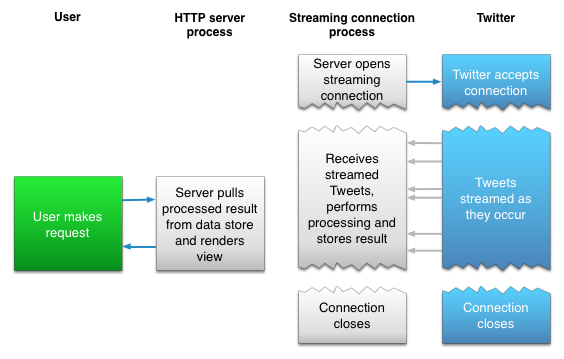
\includegraphics[width=10cm]{../images/twitter_streaming_diagram.png}
\end{figure}

Twitter itself offers 6 different endpoints for 6 different streams, all of which are explained in~\autoref{tab:twitter_streams}.

\begin{table}
    \caption{All streams offered by Twitter~\cite{twitterDocs}}
    \label{tab:twitter_streams}
    \resizebox{\textwidth}{!}{%
    \begin{tabular}{llllll} %
        \toprule
        & & & \multicolumn{2}{c}{Authentication} \\
        \cmidrule{4-5}
        Name
        & Method
        & URI
        & User
        & Application
        & Description
        \\
        \midrule
        Filter stream
        & \texttt{POST}
        & \texttt{statuses/filter}
        & \cmark
        & \cmark
        & Streams a random sample of statuses matching the filter setting
        \\
        \midrule
        Sample stream
        & \texttt{GET}
        & \texttt{statuses/sample}
        & \cmark
        & \cmark
        & Streams a random sample of statuses
        \\
        \midrule
        User stream
        & \texttt{GET}
        & \texttt{user}
        & \cmark
        & \xmark
        & Streams all activity regarding the authenticated user
        \\
        \midrule
        Site stream
        & \texttt{GET}
        & \texttt{site}
        & & &
        \\
        \cmidrule{1-3}
        Retweet stream
        & \multicolumn{2}{c}{\textit{Unknown}}
        & \multicolumn{3}{c}{Not publicly available, disregarded}
        \\
        \cmidrule{1-3}
        Firehose
        & \multicolumn{2}{c}{\textit{Unknown}}
        & & &
        \\
        \bottomrule
    \end{tabular}}
\end{table}

This thesis will work with the sample- and filter-stream, since only these are publicly available and do not depend on a specific user,
to give reproducible results.
The main focus will be the sample stream, since it gives a representative sample of all activity on Twitter.
While these streaming endpoints are not rate limited in the number of entities streamed,
they are limited in regards to the number of connection requests any one user or application can make.
To give a feeling for the rate at which statuses will need to be analyzed,
the number of statuses per second for two different streams were recorded over a 10 second period.
The first stream was the sample stream, with the language set to english.
The second stream was the filter stream, tracking only the keyword \texttt{iPhone}, and the language also set to english.
The data was recorded on the 30$^th$ of September 2017.
The results can be seen in~\autoref{fig:stream_frequency}.

% include diagram
\begin{figure}
    \centering
    \caption{The number of incoming statuses per second for 2 different streams}
    \label{fig:stream_frequency}
    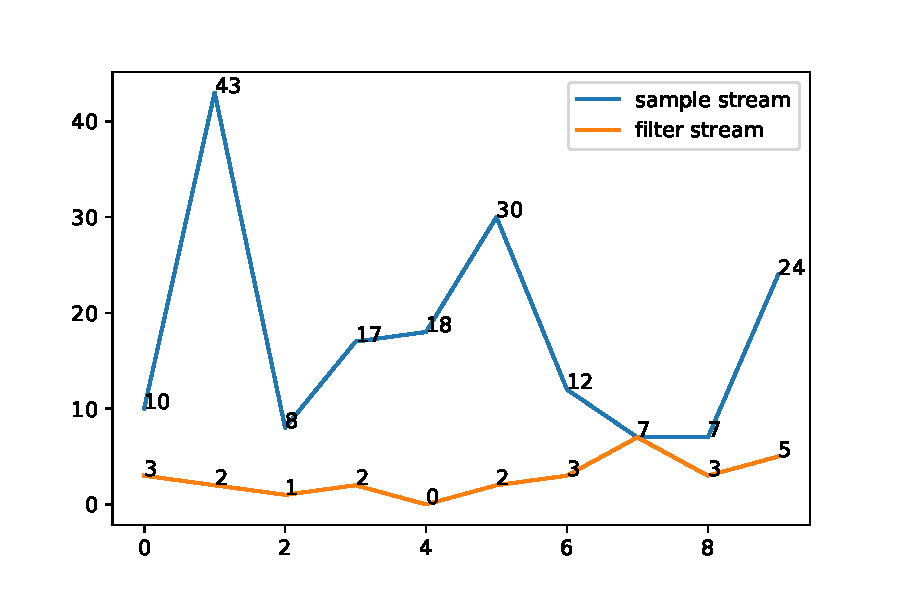
\includegraphics[width=10cm]{../figures/stream_frequencies.pdf}
\end{figure}

It has to be noted that the results are not representative of the share of statuses containing the keyword \texttt{iPhone},
since the Twitter streaming API only sends an indeterminate, small part of all statuses posted~\cite{twitterDocs}.

\par
Compared to the general use-case for Kafka shown in~\autoref{fig:kafka}, in this thesis,
every producer will produce events for exactly one topic, with the producer being a specific Twitter stream and the topic beint a unique identifier for it.
The advantage of using the Twitter streaming-API compared to repeatedly polling the REST-API for the use-case of this thesis
is that it is more efficient and has less latency.

\section{The Sanders Dataset}
\label{sec:theSandersDataset}

Since the model used for sentiment analysis will be trained using a supervised approach,
a set of statuses labeled with sentiment was needed.
Evaluation using the comparison in~\cite{Saif2013} showed the Sanders-dataset~\cite{sanders} to be most-suited to train Twitter sentiment analysis models.
At 4347 available statuses, it is large enough to train an accurate model and is hand-labeled instead of relying on, for example, emoticons for labeling, which might be flawed.
Also, Twitter's terms of service forbid the distribution of statuses outside of their API, which ruled out all datasets that did.
Even though the NLTK~\autoref{subsec:nltk} contains a Twitter sentiment sample dataset,
there is no information available on how it was collected and labeled, which is why it wasn't considered.
The Sanders-dataset only contains the statuses unique identifier (id), along with the sentiment label ("positive", "negative", "neutral" or "irrelevant").
The existing scripts to hydrate the dataset (meaning to replace the id with the actual status by requesting them from the API) were either slow or deprecated and dysfunctional,
which is why a new script was written.
Unfortunately, due to Twitter's terms of service, no real statuses can be shown, but~\autoref{tab:sanders_sample} shows some fictional examples.

\begin{table}
    \caption{Some fictional statuses with labels}
    \label{tab:sanders_sample}
    \centering
    \begin{tabular}{lllll} %
        \toprule
        Text
        & Sentiment Label
        \\
        \midrule
        Lmao I had a funny argument with Siri @Apple
        & \texttt{positive}
        \\
        My \#iPad crashes constantly since the update.
        & \texttt{negative}
        \\
        Can anyone recommend me an app for my iPhone?
        & \texttt{neutral}
        \\
        Apple stellt neues iPhone vor \textit{(non-english)}
        & \texttt{irrelevant}
        \\
        \bottomrule
    \end{tabular}
\end{table}

The resulting dataset was then filtered to only contain english statuses, which left 2946 statuses.
The distribution of labels on the dataset can be seen in~\autoref{fig:sanders_sentiment}.

% include diagram
\begin{figure}
    \centering
    \caption{The distribution of labels in the Sanders dataset.}
    \label{fig:sanders_sentiment}
    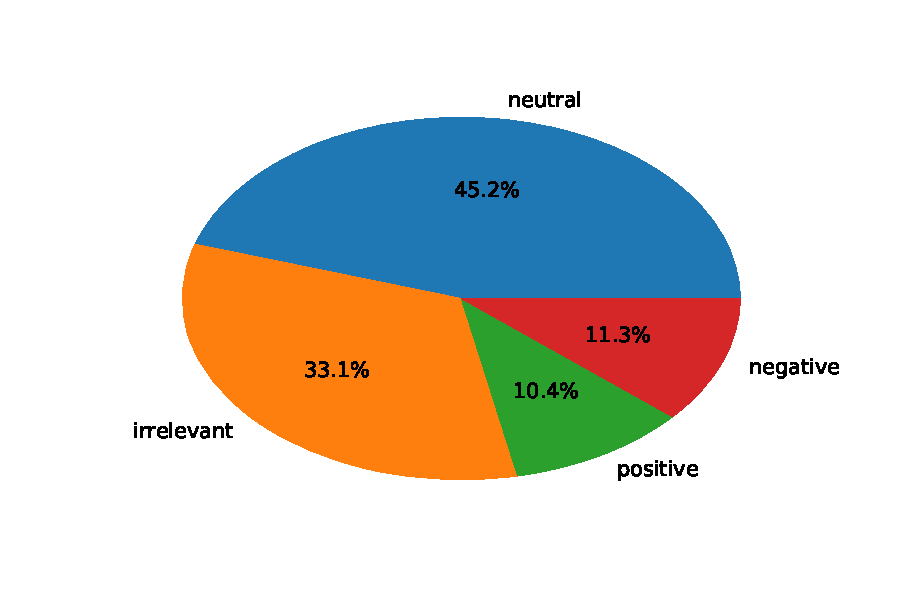
\includegraphics[width=10cm]{../figures/sanders_sentiment.pdf}
\end{figure}

The statuses were collected using the search terms "@apple", "\#google", "\#microsoft" and "\#twitter",
which not only renders them unusable to create a topic model since that makes them highly topical,
but might also negatively impact the ability of sentiment analysis models trained on them to generalize over other data.
Furthermore, of the remaining english statuses, only 431 and 481 were labeled as positive and negative respectively,
which might be too few to train an accurate model.
This will be explored further in~\autoref{ch:sentimentAnalysis}.

\section{The Streaming Sample Dataset}
\label{sec:streamingSampleDataset}

Another dataset was collected by streaming the sample stream described in~\autoref{subsec:streaming},
again only keeping english tweets.
The statuses were collected on the 18$^{th}$ of august 2017.
The statuses received via the stream were written to a database until 7000 statuses were collected.
This dataset will be used for (unsupervised) topic modeling, since it is representative of all activity on Twitter.
A wordcloud of the statuses collected from the sample stream can be seen in~\autoref{fig:wordloud_pre}.

% include diagram
\begin{figure}
    \centering
    \caption{Wordcloud of the statuses collected from the sample stream.}
    \label{fig:wordloud_pre}
    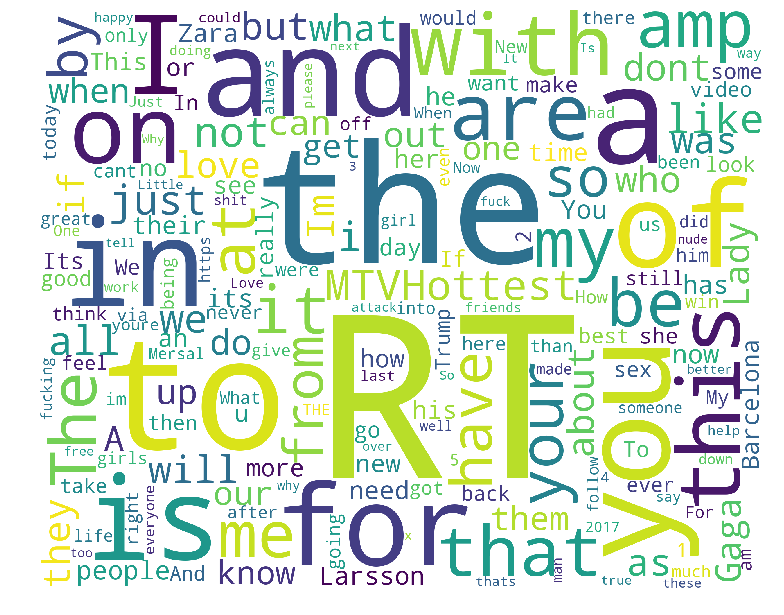
\includegraphics[width=12cm]{../images/wordcloud_pre.png}
\end{figure}

Some of the biggest "words" in the wordcloud are "RT", "it" and "be",
or even some digits, which have no informativeness with regards to sentiment or topic,
demonstrating the necessity of preprocessing, shown in the next chapter.

\section{Preprocessing and Tokenization}
\label{sec:preprocessingAndTokenization}

There are now 2 datasets of statuses that are filtered by language but still raw.
Since the quality of the results will depend on the quality of the data,
these datasets now need to be preprocessed.
In this case that means removing all elements of text that have no influence on topic and sentiment and make
modeling and analysis unnecessarily difficult.\\
Furthermore, since all the algorithms that will be used later on are bag-of-words algorithms,
which means they disregard the order of words in text, a tokenization function needs to be created
to split sentences in the right places and only keep tokens (terms, words) relevant for modeling and analysis.
\\
At this point it is important to mention that while the tokenization does not, strictly speaking, tokenize the documents,
but rather splits them into terms, this thesis will stick to the NLTK's~\cite{nltkDocs} nomenclature, and call the terms tokens.
\\
To achieve consistent results, the same preprocessing and tokenization functions need to be used for all models, analyses and datasets.
The following steps were taken.

\begin{enumerate}
    \item Preprocessing
    \begin{enumerate}
        \item All URL's were removed by using a regular expression matching everything from "http" up to the next whitespace
        \item All punctuation as well as the Twitter-specific characters \texttt{@} and \texttt{\#} were removed
        \item The text was split at whitespace using the \texttt{\\s} regular expression
        \item All elements that contained anything but latin letters were discarded
    \end{enumerate}
    \item Tokenization
    \begin{enumerate}
        \item The text is split into tokens using the whitespace regular expression again
        \item Terms of length 1 are removed
        \item Terms that can be found in NLTK's stopwords list for the english language
        (containing a fixed selection of terms with low informativeness for bag-of-words algorithms),
        were removed. \textit{(This only applies to topic modeling)}
        \item Terms that can be found in an additional self-devised stopwords list specific to this case were removed
    \end{enumerate}
\end{enumerate}

The Python implementation of these functions can be found in the Appendix in~\autoref{sec:preprocessingAndTokenizationFunctionFactories}.
\par
While some approaches to removing terms with low informativeness rely on removing terms that occur in too many or too few documents,
in this thesis, a stopword list is used,
since only english statuses will be considered, and extensive stopword lists exit for the english language~\cite{Porter2001}.
The change to the wordcloud of the statuses collected from the sample stream after preprocessing and tokenization (including stopword removal) can be seen in~\autoref{fig:wordloud_post}.

\begin{figure}
    \centering
    \caption{Wordcloud of the statuses collected from the sample stream after preprocessing and tokenization.}
    \label{fig:wordloud_post}
    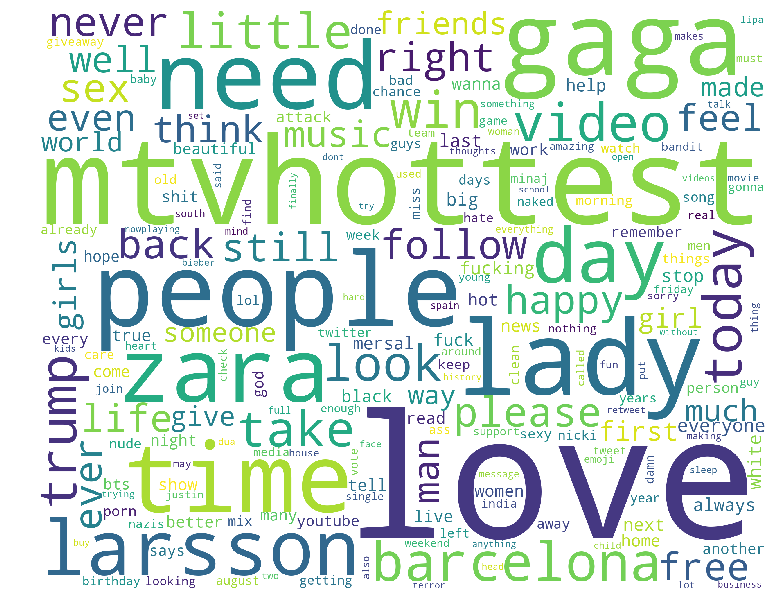
\includegraphics[width=12cm]{../images/wordcloud_post.png}
\end{figure}
% !TEX root = ../main.tex
\chapter{Sentiment Analysis}
\label{ch:sentimentAnalysis}

% TODO redo all of these analyses, filter out non-english tweets for all these
Semantic orientation describes the strength and polarity of words and phrases used in text.
Extraction of subjectivity and polarity of the text from the semantic orientation of its words and phrases is called sentiment analysis.
The huge volume of text-based interactions on social media make it difficult
to read and organize them and analyze their sentiment by humans.
Focusing on single instances of interaction also makes it difficult to extract the overall sentiment,
necessitating a solution that performs and summarizes the analysis automatically, fast, and gives human-comprehensible results~\cite{Sarlan2014}.

\section{Methods}
\label{sec:methods}

The informal language used in statuses on Twitter, and the limited length, poses an additional difficulty
to analyzing their sentiment.
Previous research showed supervised approaches, as opposed to lexicon-based approaches, to be superior~\cite{Sarlan2014}.
Since labeled data is available from the Sanders dataset~\ref{sec:theSandersDataset},
this thesis will focus on supervised approaches.
The dataset was preprocessed using the preprocessing and tokenization functions introduced in~\ref{sec:preprocessingAndTokenization} (without stopwords removal).

\subsection{Na\"{i}ve Bayes}
\label{subsec:naivebayes}

The naive Bayes algorithm works by first expressing the probability of a label given the features,
in this case the sentiment given the bag of words that is the status, with Bayes rule:

\begin{math}
    P(label|features) = \frac{P(label)*P(features|label)}{P(features)}
\end{math}

The algorithm then naively assumes that all features are independent, giving:

\begin{math}
    P(label|features) = \frac{P(label)*P(feature 1|label)*...*P(feature n|label)}{P(features)}
\end{math}


The denominator $P(features)$ is not explicitly calculated.
Instead, all numerators are calculated and the denominator is chosen such that all $P(label|features)$ sum to 1~\cite{nltkDocs}.
\\
The features of each status are extracted as a vector of every distinct word in the dataset,
together with $True$ if the word can be found in the status, or $False$ if not.
The Python-code achieving this encoding can be seen in~\ref{code:extract_features}.

\begin{figure}
    \caption{Encoding a status as a vector.}
    \label{code:extract_features}
    % @formatter:off
    \begin{minted}{python}
features = {} # Contains every word in the dictionary and whether the status contains it.
# Using the previously created dictionary
for word in dictionary:
    features['contains(\%s)' \% word] = (word in document_words)
    \end{minted}
    % @formatter:on
\end{figure}

NLTK's implementation of this algorithm is used~\cite{nltkDocs}.
This implementation assumes the distribution of each feature $P(feature i|label)$ to be multinomial,
making it a multinomial naive Bayes, which has shown the best performance in previous work~\cite{Go2009}.
The data from the hydrated Sanders dataset created in~\ref{sec:theSandersDataset} was shuffled and split into $10\%$ test data and $90\%$ training data.
This classifier achieved an accuracy of $74\%$.
In addition to accuracy, the performance measures precision, recall and F-measure,
the definition of which can be seen in~\ref{math:precision_recall_fmeasure}, were computed.

\begin{figure}
    \caption{Definition of precision, recall and F-measure~\cite{Hong2010}.}
    \label{math:precision_recall_fmeasure}
    \begin{math}
        p_t = number of true positives
        p_f = number of false positives
        n_t = number of true negatives
        n_f = number of false negatives
        \\
        Precision = \frac{p_t}{p_t + p_f}
        Recall = \frac{p_t}{p_t + n_f}
        \\
        F-Measure = \frac{2 \* Precision \* Recall}{Precision + Recall}
    \end{math}
\end{figure}

Intuitively, precision and recall can be understood the percentage of positives that are real positives,
and the percentage of real positives that were labeled as positives, respectively.
The F-measure is their harmonic mean.
The measures, for each sentiment-class, can be seen in~\ref{tab:mnb_results}.

\begin{table}
    \caption{Sentiment classification results using multinomial naive Bayes}
    \label{tab:mnb_results}
    \resizebox{\textwidth}{!}{%
    \begin{tabular}{llll} %
        \toprule
        Sentiment
        & F-measure
        & Precision
        & Recall
        \\\midrule
        neutral & 0.769 & 0.747 & 0.792
        \\\midrule
        irrelevant & 0.896 & 0.902 & 0.890
        \\\midrule
        negative & 0.504 & 0.464 & 0.553
        \\\midrule
        positive & 0.318 & 0.440 & 0.250
        \\\bottomrule
    \end{tabular}}
\end{table}

% TODO maybe a bit of interpretation
Class distribution and absolute counts for each class can be seen in~\ref{tab:naive_bayes_results}.

\begin{table}
    \caption{Sentiment classification using multinomial naive Bayes}
    \label{tab:naive_bayes_results}
    \resizebox{\textwidth}{!}{%
    \begin{tabular}{lllll} %
        \toprule
        & \multicolumn{2}{c}{Test Data} & \multicolumn{2}{c}{Classification Result}\\
        \cmidrule{3-4}
        Sentiment
        & Count
        & Percentage
        & Count
        & Percentage
        \\\midrule
        neutral & 206 & 47\%  & 266 & 61\%
        \\\midrule
        irrelevant & 146 & 33\%  & 124 & 28\%
        \\\midrule
        negative & 42 & 9\%   & 30 & 6\%
        \\\midrule
        positive & 41 & 9\%   & 15 & 3\%
        \\\bottomrule
    \end{tabular}}
\end{table}

When the dictionary created from the sample stream was used to extract the features as shown in~\ref{code:extract_features},
the accuracy dropped to $62\%$, confirming that the Sanders dataset, and the dictionary created from it, is highly topical.

\subsection{NLTK Sentiment Analyzer}
\label{subsec:nltksentimentanalyzer}

The NLTK sentiment analyzer package provides a framework for building classification-pipelines with easily interchangeable components
(like choosing which methods to use for training, or which feature extractors to use).
It also builds its own dictionary, which means the dictionary created in~\ref{sec:preprocessingAndTokenization} doesn't need to be used.
\par
First, the previous approach was reconstructed in this framework, and successfully validated to give the same accuracy.
Then, it was expanded by marking all negated words as negated using the \texttt{mark\_negation} utility function of the NLTK.
They were then added to the dictionary in their negated form.
\\
This yielded no performance increase.
\\
Inspection revealed that only 22 words were added to the dictionary in negated form.
Since the tokenization function described in~\ref{sec:preprocessingAndTokenization} filters tokens of length shorter then 3,
thereby also filtering, for example, the word "no", another test was conducted with a modified tokenization function that doesn't filter out short words.
\\
This also yielded no performance increase.
\\
Only two more distinct words were found in their negated form and added to the dictionary,
increasing the dictionary size of the modified tokenization function by 24, from 4132 to 4156.
\\
While recognizing contextual polarity has shown improvements in accuracy in a more general case~\cite{Hoffmann2005},
these results indicate that marking negated words does not have the same positive effect on the special case presented by Twitter statuses.

\subsection{VADER}
\label{subsec:vader}

% TODO Interestingly, Vader performs better on the dataset provided by the nltk (which is collected using...) than the sanders-dataset
VADER (\textbf{V}alence \textbf{A}ware \textbf{D}ictionary for s\textbf{E}ntiment \textbf{R}easoning))
is a gold standard of lexical features together with five general rules embodying grammatical and syntactical conventions
that were devised in a human-centered approach.
It is specifically designed for microblog-like environments such as Twitter~\cite{Hutto2014}.
\par
NLTK's implementation of VADER returns scores between 0 and 1 for positivity, negativity and neutrality,
as well as a compound score between -1 and 1, where the direction represents polarity and the magnitude represents subjectivity.
A test was conducted involving only the statuses labeled "positive", "negative" or "neutral",
to avoid the ambiguity of the "irrelevant"-label.
The optimal threshold for which a status will be classified as neutral was chosen
at an absolute value for the compound score of 0.8, giving an accuracy of 68\%.
% TODO insert {-bracketed mathematical respresentation of that here
Still, this accuracy remained below that of the naive Bayes approach at 75\% when using the same, filtered statuses.
Detailed results can be seem in~\ref{tab:vader_results}.

\begin{table}
    \caption{Sentiment classification using VADER}
    \label{tab:vader_results}
    \resizebox{\textwidth}{!}{%
    \begin{tabular}{llll} %
        \toprule
        Sentiment
        & F-measure
        & Precision
        & Recall
        \\\midrule
        neutral & 0.806 & 0.689 & 0.971
        \\\midrule
        negative & 0.098 & 0.742 & 0.052
        \\\midrule
        positive & 0.171 & 0.448 & 0.105
        \\\bottomrule
    \end{tabular}}
\end{table}

\subsection{TextBlob}
\label{subsec:textblob}

TextBlob is a simple text-processing library written in Python.
It provides similar functionality than the NLTK described in~\ref{subsec:nltk},
but is simpler and less extensive.
Among other, it offers sentiment analysis~\cite{textblobDocs}.
TextBlob returns a polarity score between -1 and 1 as well as a subjectivity score between 0 and 1.
As in the previous subsection, the Sanders dataset is used for evaluation, disregarding statuses labeled as irrelevant.
A scatter plot of the polarity and subjectivity score on the axes and label represented as the color can be seen in~\ref{fig:textblob}.


\begin{figure}
    \centering
    \caption{Scatter plot of the polarity and subjectivity score computed by TextBlob on the axes and label represented as the color.}
    \label{fig:textblob}
    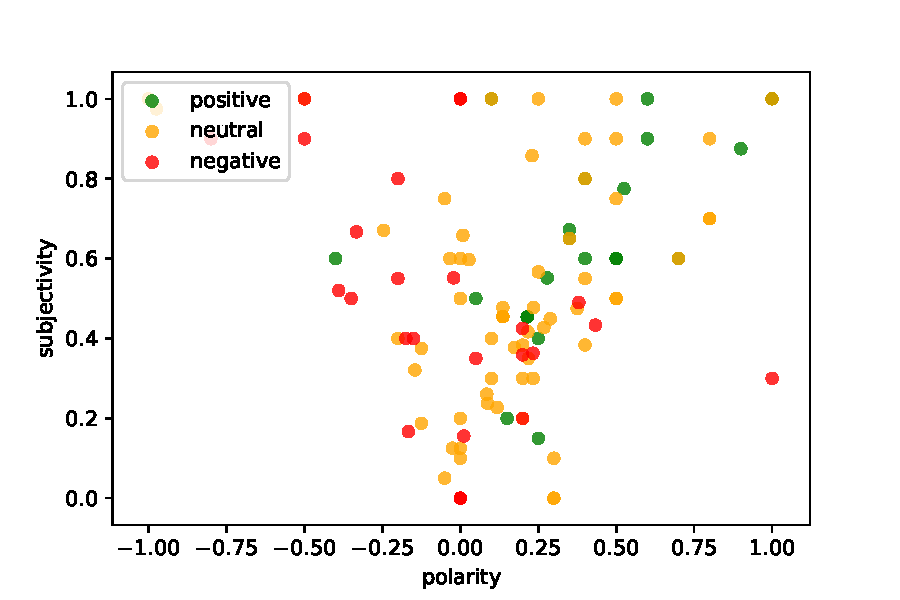
\includegraphics[width=10cm]{../figures/textblob.pdf}
\end{figure}

The plot clearly shows the algorithms incapability of distinguishing subjective from neutral statuses,
which is why a quantitative accuracy test was conducted using only tweets labeled as negative or positive.
% TODO insert {-bracketed mathematical respresentation of that here
The TextBlob's sentiment analysis algorithm achieved an accuracy of 64\% on this filtered dataset,
whereas the current frontrunner, the multinomial naive bayes, achieved an accuracy of 72\% on the same filtered dataset.

\subsection{Google Cloud}
\label{subsec:googlecloud} % TODO korrekte Bezeichnung

The natural language API by Google Cloud offers sentiment analysis as a service.
For any documented, provided in a supported language, the API returns a magnitude starting from 0 with an undocumented upper bound
(although the highest observed was 4.1) and a score between -1 and 1.
Magnitude and subjectivity as well as score and polarity are similarly described in the their relative documentation~\cite{gcloudDocs}\cite{textblobDocs}.
\par
The API is billed on a per-request basis, so all statuses from the Sanders dataset were classified once and persisted in a CSV-file.
Again, statuses labeled as irrelevant were filtered out to avoid ambiguity.
A scatter plot of the score and magnitude on the axes and label represented as the color can be seen in~\ref{fig:gcloud}.

\begin{figure}
    \centering
    \caption{Scatter plot of the score and magnitude computed by the Google Cloud natural language API on the axes and label represented as the color.}
    \label{fig:gcloud}
    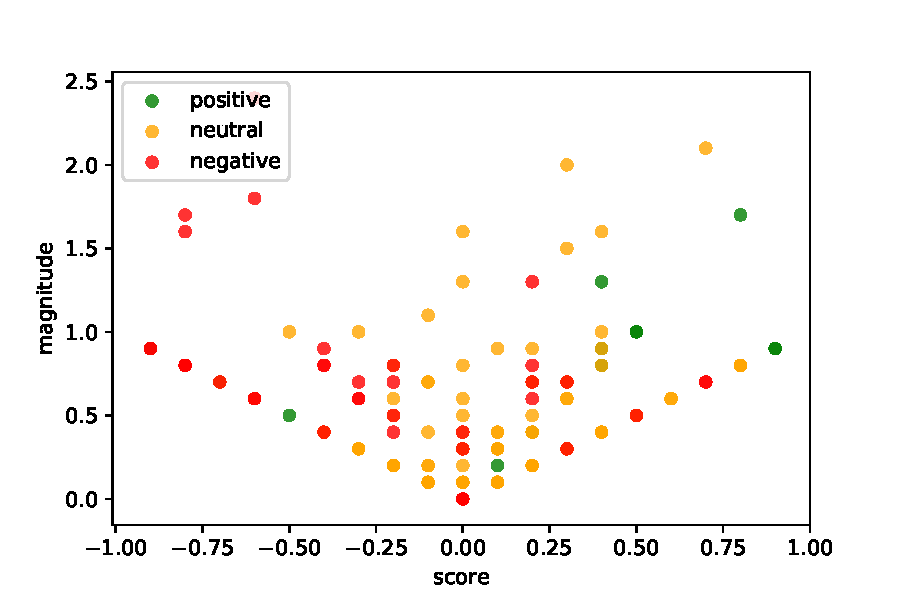
\includegraphics[width=10cm]{../figures/gcloud.pdf}
\end{figure}

As for the VADER-classifier in~\ref{subsec:vader}, these values are mapped to the labels from the dataset by
choosing an optimal threshold for which a status will be classified as neutral.
The optimal magnitude-threshold was found at a magnitude of 0.9, giving an accuracy of 49\%,
which is just marginally better than guessing neutral, with 47\% of statuses being labeled neutral.
Without neutral-labeled statuses, an accuracy of 73\% was achieved.

\section{Comparison and Conclusion}
\label{sec:comparison}

When comparing the results of the different methods presented, it is suprising to see the simplest,
a multinomial naive Bayes, turned out to be most accurate.\\
This indicates that short text statuses on micro-blogs like Twitter present a special challenge to sentiment analysis
that cannot be solved with current approaches.
Additions to existing algorithms, like marking negated words, that showed improved results with regular texts,
showed no improvement to the multinomial naive Bayes classifier when working with Twitter statuses.
Furthermore, even methods specifically designed for this special challenge, like VADER,
were outperformed by a multinomial naive Bayes classifier.
\par
However, the results of these tests need to be handled carefully,
since the training dataset is highly topical as shown by the performance discrepancies between different dictionaries in~\ref{subsec:naivebayes}.
\par
The multinomial naive Bayes classifer created in~\ref{subsec:naivebayes} was saved and will be used in the coming chapters.

% !TEX root = ../main.tex
\chapter{Topic Modeling}
\label{ch:topicModeling}

Topic models are probabilistic models which are used to extract an underlying semantic structure from text artifacts, or documents.
They are based on a hierarchical bayesian analysis on the terms in a document,
on which a similarity measure for the its content can be defined and used to "connect" and cluster documents.

Topic models are useful when dealing with large quantities of unstructured documents,
that need to be automatically structured, grouped or filtered for knowledge extraction,
for example to provide similar/related content at the end of blog entries,
or to automatically tag content with relevant keywords~\cite{blei2009topic}.

In this chapter, methods for topic modeling will be explored,
and a suitable model for the use-case of this thesis will be determined.
While it is easy for humans to gain an intuitive understanding what a document is about
and other subjective attributes, machines lack this intuition.
Therefore, the topic modeling methods presented in this chapter infer \textit{latent} topics,
meaning that they are unable to name or describe a topic, but merely confirm its existence.
However, since the topics inferred are dependent on term (in this case: word) frequencies,
the models can provide a human-understandable representation of a topic by listing its most frequent terms.

\section{Methods}
\label{sec:methods_topicmodeling}

Similar to the previous chapter, multiple methods to perform topic modeling will be explained and demonstrated.
However, since no labeled dataset of a representative sample of statuses on Twitter and their respective topics is available,
only subjective assessments can be made to their performance.
Although the Sanders-dataset was collected by filtering a stream for specific keywords as described in~\cref{sec:theSandersDataset},
and these could be used as labels for a supervised approach such as supervised LDA~\cite{Blei2008},
the dataset is not representative of all activity on Twitter and not suitable for training such a model.
Therefore, only unsupervised approaches will be considered,
and subjective choices will be made as to what constitutes a "topic" in the context of this thesis,
with the parameters for the models being determined accordingly.

\subsection{TF-IDF}
\label{subsec:tfidf}

Both algorithms use TF-IDF (\textbf{T}erm \textbf{F}requency - \textbf{I}nverse \textbf{D}ocument \textbf{F}requency).
In the TF-IDF scheme, first, a dictionary of terms (words, usually) that the documents are made of is formed.
In this case, this dictionary will be created by taking all the terms (words) in the dataset,
and removing those that occur only once, to reduce its size.
Also, contrary to~\cref{ch:sentimentAnalysis}, in this chapter,
the tokenization function will also remove stopwords, as described in~\cref{sec:preprocessingAndTokenization}.
Another strategy that could've been used for scenarios where comprehensive stopword lists are not available
would be to remove a percentage or absolute number of most and least frequent terms,
which have little informativeness since they occur in too many or too few documents.
The implementation of the dictionary creation process can be seen in~\cref{code:create_corpus}.

\begin{figure}
    \caption{Implementation of corpus-creation}
    \label{code:create_corpus}
    % @formatter:off
    \begin{minted}{python}
        # The usual preprocessing and tokenization
        tweets = [tokenize(preprocess(tweet) for tweet in tweets]

        # Count term occurences
        term_count_dictionary = defaultdict(int)
        for tweet in tweets:
            for term in tweet:
                term_count_dictionary[term] += 1

        # keep terms that occur more than once
        terms = [[(term, term_count_dictionary[term]) for term in tweet
                if term_count_dictionary[term] > 1] for tweet in tweets]
    \end{minted}
    % @formatter:on
\end{figure}

To compute the TF-IDF values for a specific document,
a term count vector is then formed containing how often each term in the dictionary occurs in that document,
and normalized over the length to result in the frequency.
This is usually sparsely implemented, since especially with short Twitter statuses,
most words in the corpus do not occur in the document.
Also, since some words might generally occur more often, thereby being less informative of the topic,
the frequency for each term in the document is then divided by the frequency of that term in the dictionary,
giving $term frequency / document frequency$, or $term frequency \* inverse document frequency$ (TF-IDF)~\cite{Blei2003}.

The gensim library was used to create and save the TF-IDF model,
which contains rows with two term identifiers (the terms themselves are saved in the dictionary) and a count of how often
they cooccurr in any of the training documents, while omitting term-combinations that never coocurr, to reduce size~\cite{gensimDocs}.

\subsection{LDA}
\label{subsec:lda}

The basic idea behind LDA (\textbf{L}atent \textbf{D}irichlet \textbf{A}llocation) is to represent documents as a distribution of (latent) topics,
each of which is characterized as a distribution over words.
This thesis will provide an outside view of this method, while explaining important hyperparameters and their impact.
LDA is a bag-of-words model, which means there are no syntax rules.\\
An LDA model takes the TF-IDF model created in~\cref{subsec:tfidf} as an input to determine the dirichlet distributions,
and two major hyperparameters, $\alpha$ and $\eta$,
both of which are parameters of the internal dirichlet-distributions.\\
$\alpha$ controls the per-document topic dirichlet distribution,
where a higher value indicates that documents tend to be a mixture of many topics,
and lower values lead to few topics with higher probability.\\
$\eta$ (also sometimes denoted $\beta$) controls the per-topic word dirichlet distribution, where, as with $\alpha$,
higher values lead to few words with high probabilities determining the topics,
and vice-versa.\\
The output is a matrix where every row represents a topic,
the columns are the terms from the dictionary,
and every element represents the probability that the word belongs to the topic,
with every column therefore adding up to 1.
When classifying a document, this matrix is used to allocate a distribution of topics for which the probability to have generated that document is maximized~\cite{Blei2003}.

%First, try the default settings
For LDA topic modeling, the gensim library was used~\cite{gensimDocs}.
The dataset used was the streaming sample dataset described in~\cref{sec:streamingSampleDataset},
since the Sanders dataset is topically not representative of Twitter, as described in~\cref{sec:theSandersDataset}.

To explore the results and determine the best hyperparameters, LDAvis was used.
LDAvis plots the topics on a 2D-scatterplot, with the axes being the top 2 principal components
in the hyperdimensional space of all topics, to visualize topic similarity and overlap~\cite{ldavis}.
It can also list the most relevant terms for each topic showing their frequencies in relation to their overall frequencies,
where relevancy is determined through a formula developed by Sievert \etAl~\cite{sievert2014ldavis},
which can be seen in~\cref{math:relevance}.

\begin{figure}
    \caption{Relevancy measure used in LDAvis, developed by Sievert \etAl~\cite{sievert2014ldavis}}
    \label{math:relevance}
    \begin{align*}
        relevance(term w | topic t) = \lambda \* p(w | t) + (1 - \lambda) \* \frac{p(w | t)}{p(w)}
    \end{align*}
\end{figure}

$\lambda$ adjusts the relative importance of words that are discriminant to a certain topic,
where 0.5 was found to be a good value.

After some exploration, the best-suited hyperparameters were chosen.
The number of topics was set to 10.
$\eta$ was set to 0.01, which also showed good results in previous Twitter topic modeling research~\cite{Hong2010}.
$\alpha$ is set to "auto", which means gensim learns it from the data provided, and proved to give better results than trial and error.
The LDAvis visualization for this model can be seen in~\cref{fig:ldavis}.

\begin{figure}
    \centering
    \caption{LDAvis visualization of the topic model trained on the sample dataset}
    \label{fig:ldavis}
    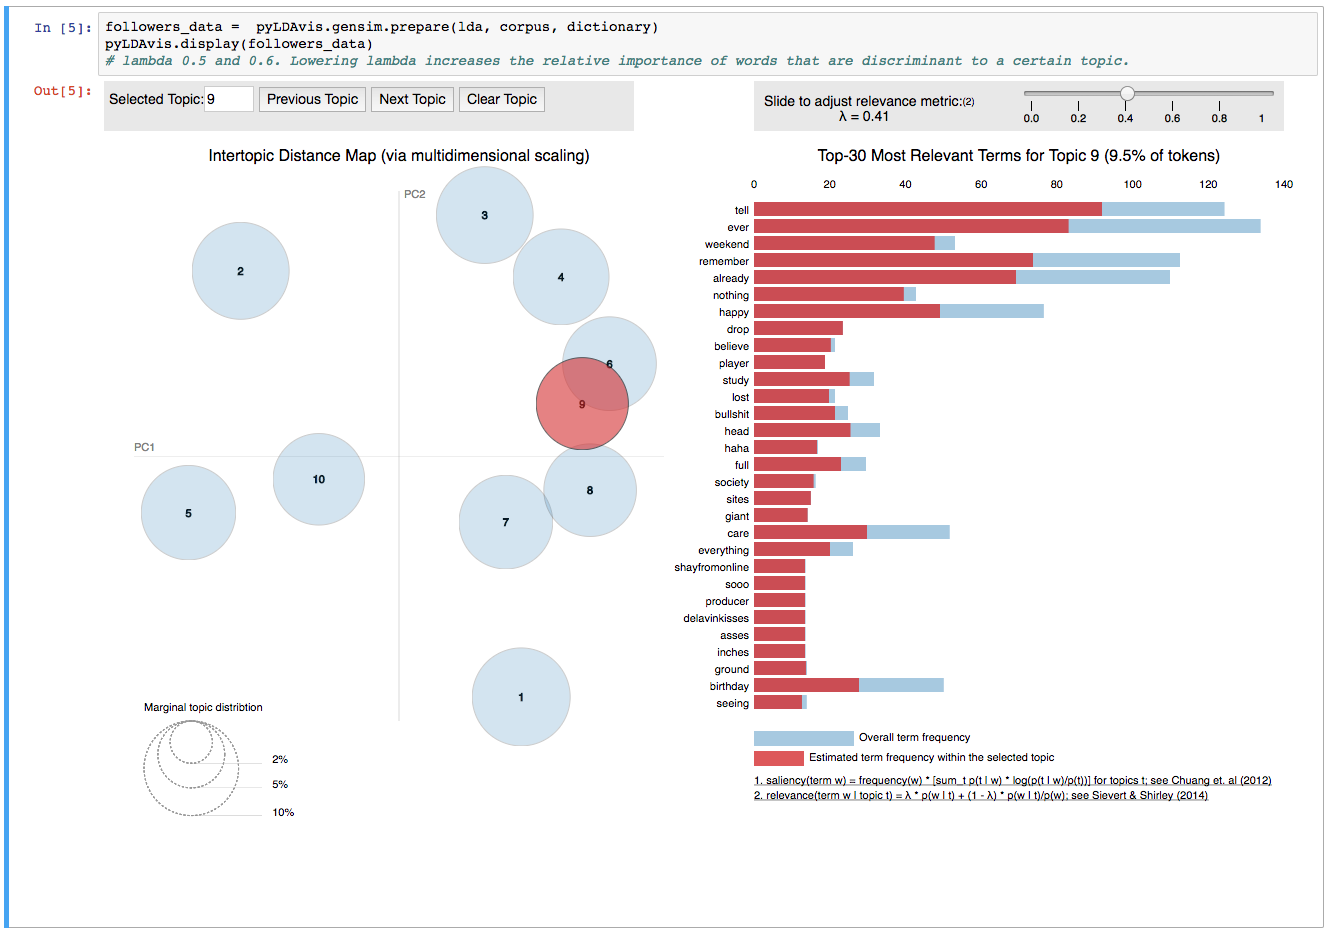
\includegraphics[width=\textwidth]{../images/LDAvis.png}
\end{figure}

Next, a different visualization, as a network graph, was devised to make a subjective assessment of the model.
In the graph, each light-blue node represents a topic.
For each topic, the 5 terms with the highest probabilities are connected with edges whose weight (thickness) represent the probability
of that word being in a document of that topic, as computed by the model.
It can be seen that some topics share terms - however, these shared terms are not very distinct terms.
The model even successfully modeled trending topics on the evening when the data was collected as described in~\cref{sec:streamingSampleDataset}.
The network graph can be seen in~\cref{fig:lda_network_graph}

\begin{figure}
    \centering
    \caption{Network graph of the LDA topic model created from the stream sample dataset}
    \label{fig:lda_network_graph}
    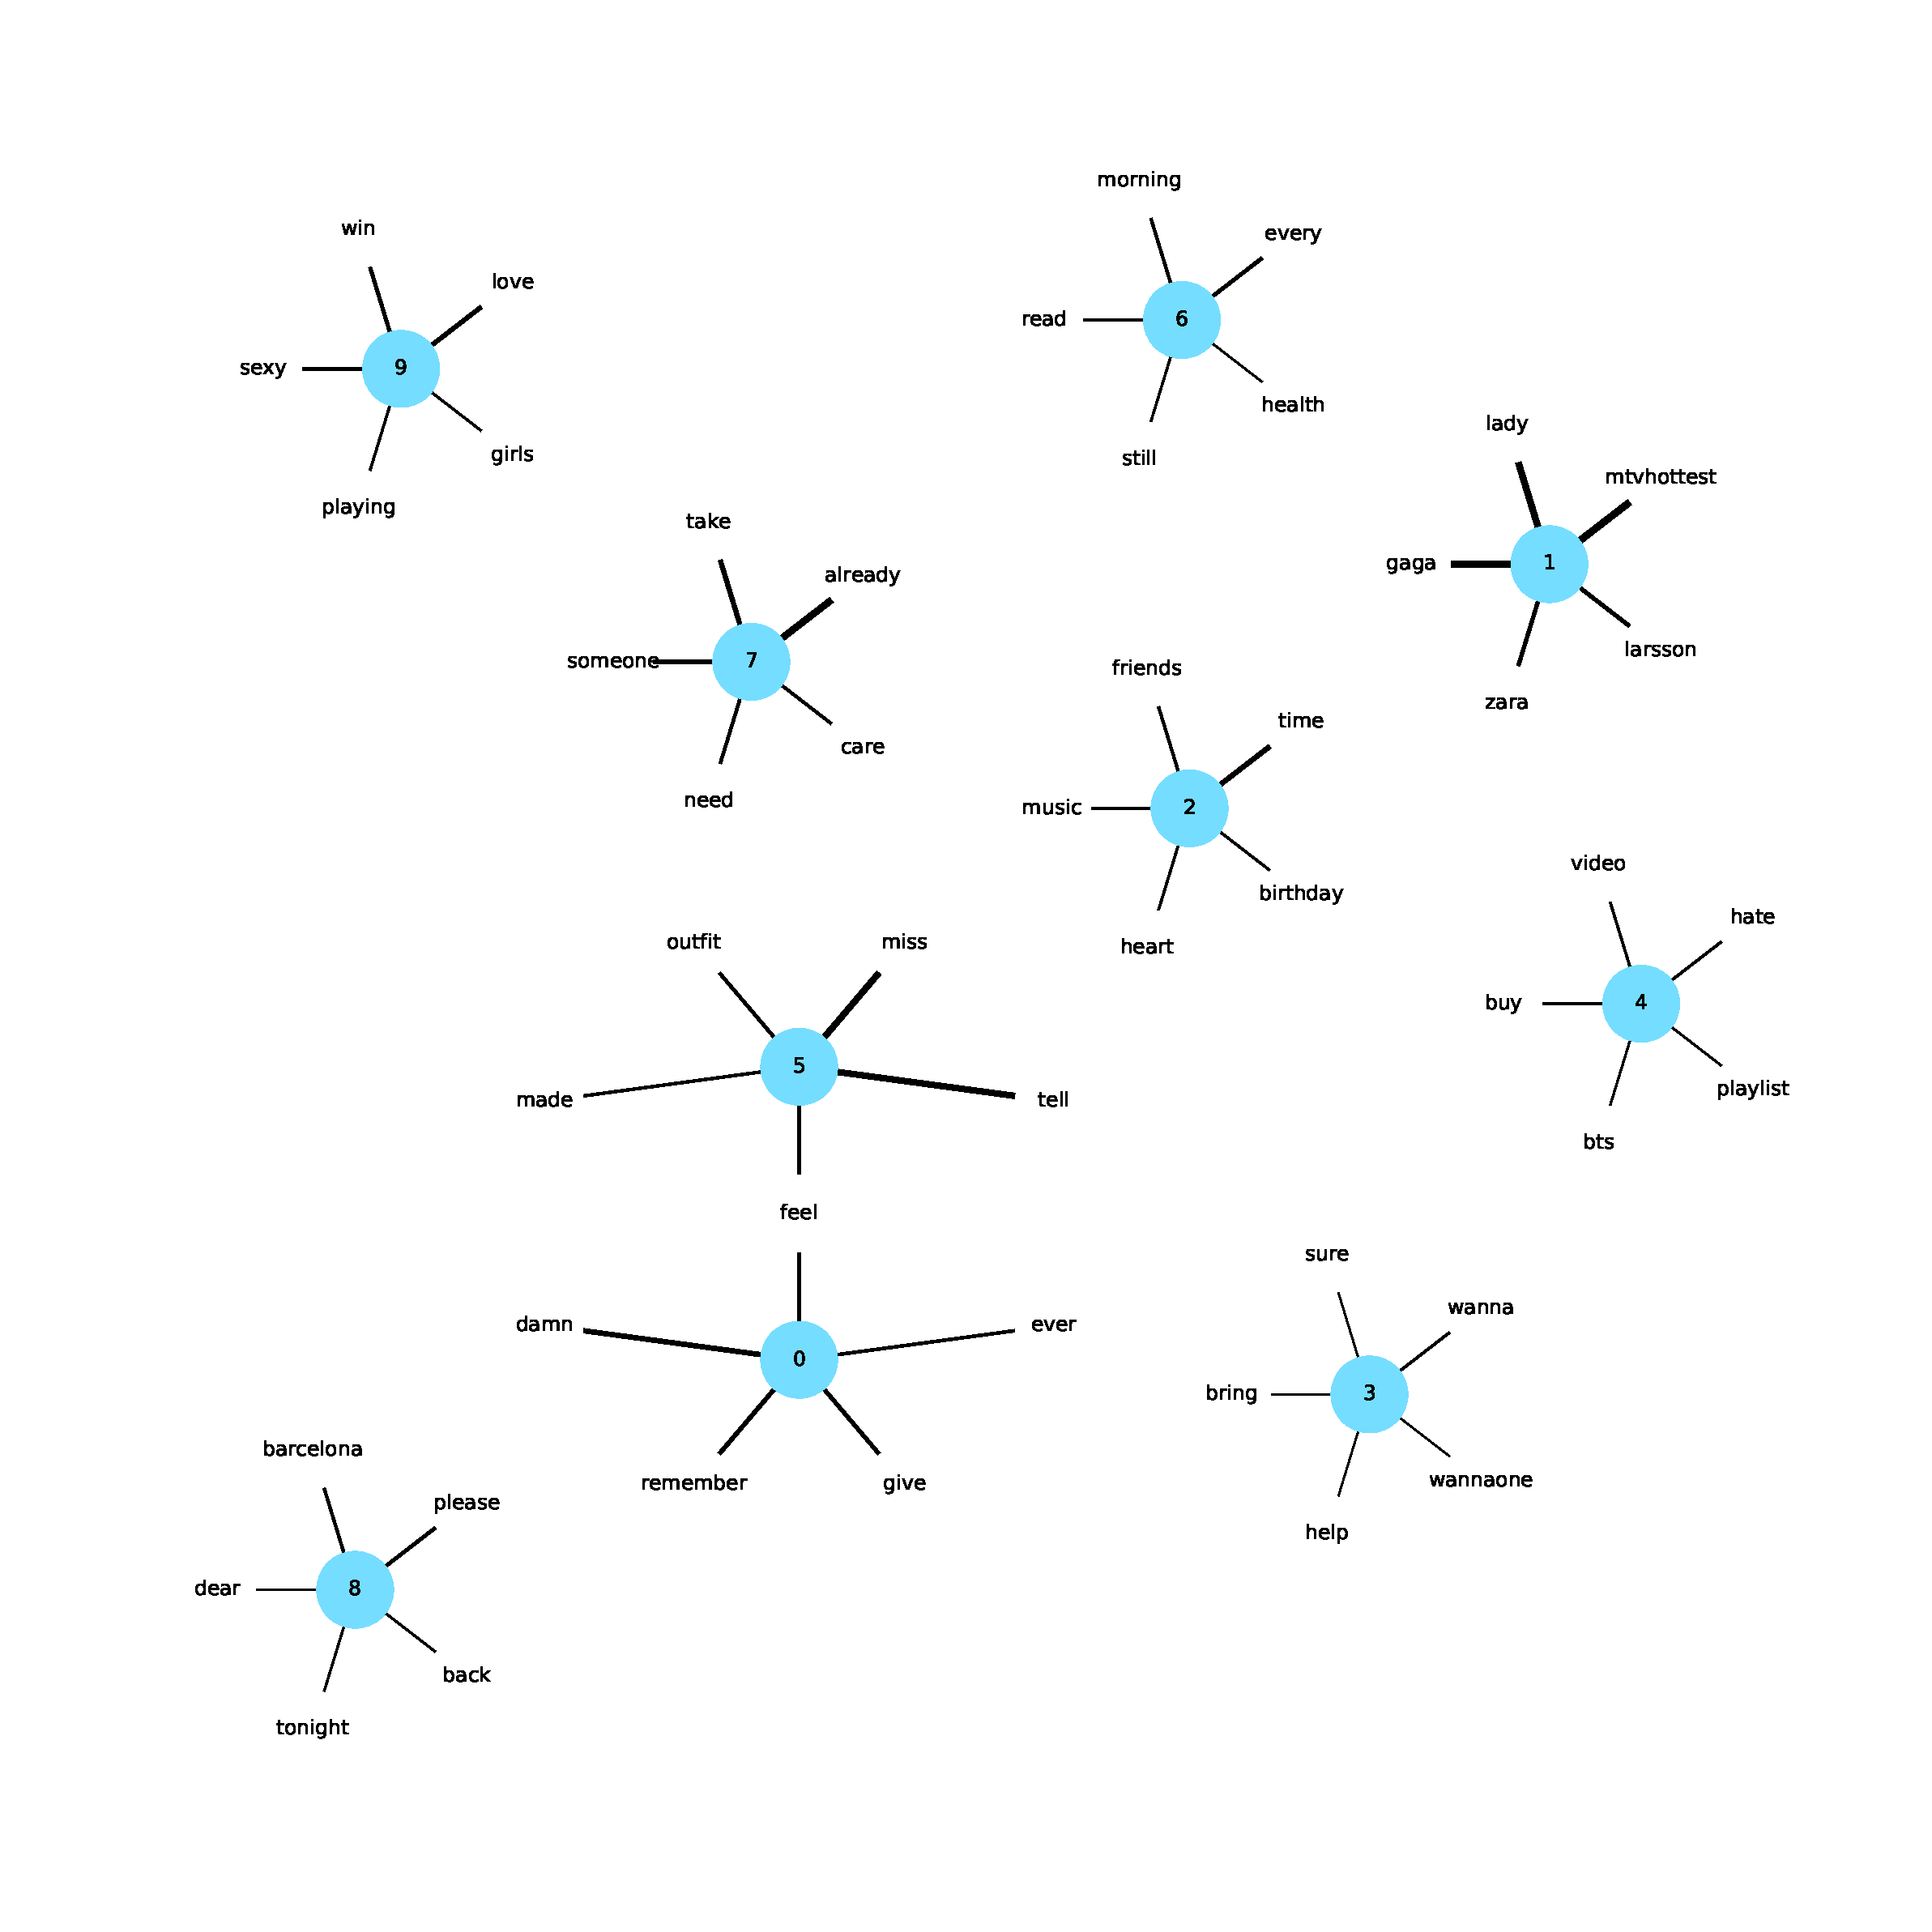
\includegraphics[width=\textwidth]{../figures/lda_network_graph.pdf}
\end{figure}

The training dataset was about equally distributed on the topic, as expected by the definition of LDA~\cite{Blei2003}.
This can be seen in~\cref{fig:sample_topic_distribution}.

\begin{figure}
    \centering
    \caption{Topic distribution of the LDA model trained on the sample dataset}
    \label{fig:sample_topic_distribution}
    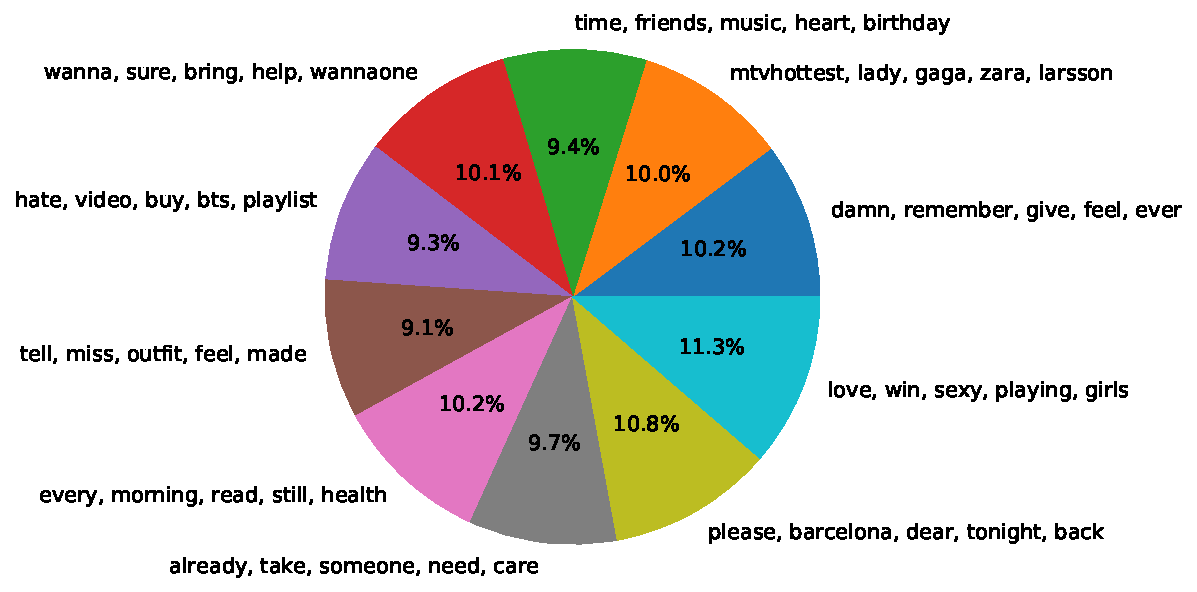
\includegraphics[width=\textwidth]{../figures/topic_distribution.pdf}
\end{figure}

\subsection{NMF}
\label{subsec:nmf}

NMF (\textbf{N}onnegative \textbf{M}atrix \textbf{F}actorization) is another active area of research in topic modeling.
It overcomes some of the shortcomings of LDA in terms of consistency across runs and empirical convergence,
since it is deterministic~\cite{Choo2013}.
It is also easier to adjust the model and incorporate feedback on the classification results in a semi-supervised approach,
making it a potentially more suitable solution for recommendation systems as described at the beginning of this chapter.
The output of the model is the same as the output of an LDA model: a term-wise representation of topics, even though the columns
do not necessarily sum up to 1.

The implementation of NMF in the scikit-learn library was used~\cite{scikitDocs}.
The number of components (the number of topics in this case) was set to 10 to ensure comparability with the LDA results.
Although several parameters were explored, the best results were accomplished with the default parameters.
The resulting network graph can be seen in~\cref{fig:nmf_network_graph}.

\begin{figure}
    \centering
    \caption{Network graph of the NMF topic model created from the stream sample dataset}
    \label{fig:nmf_network_graph}
    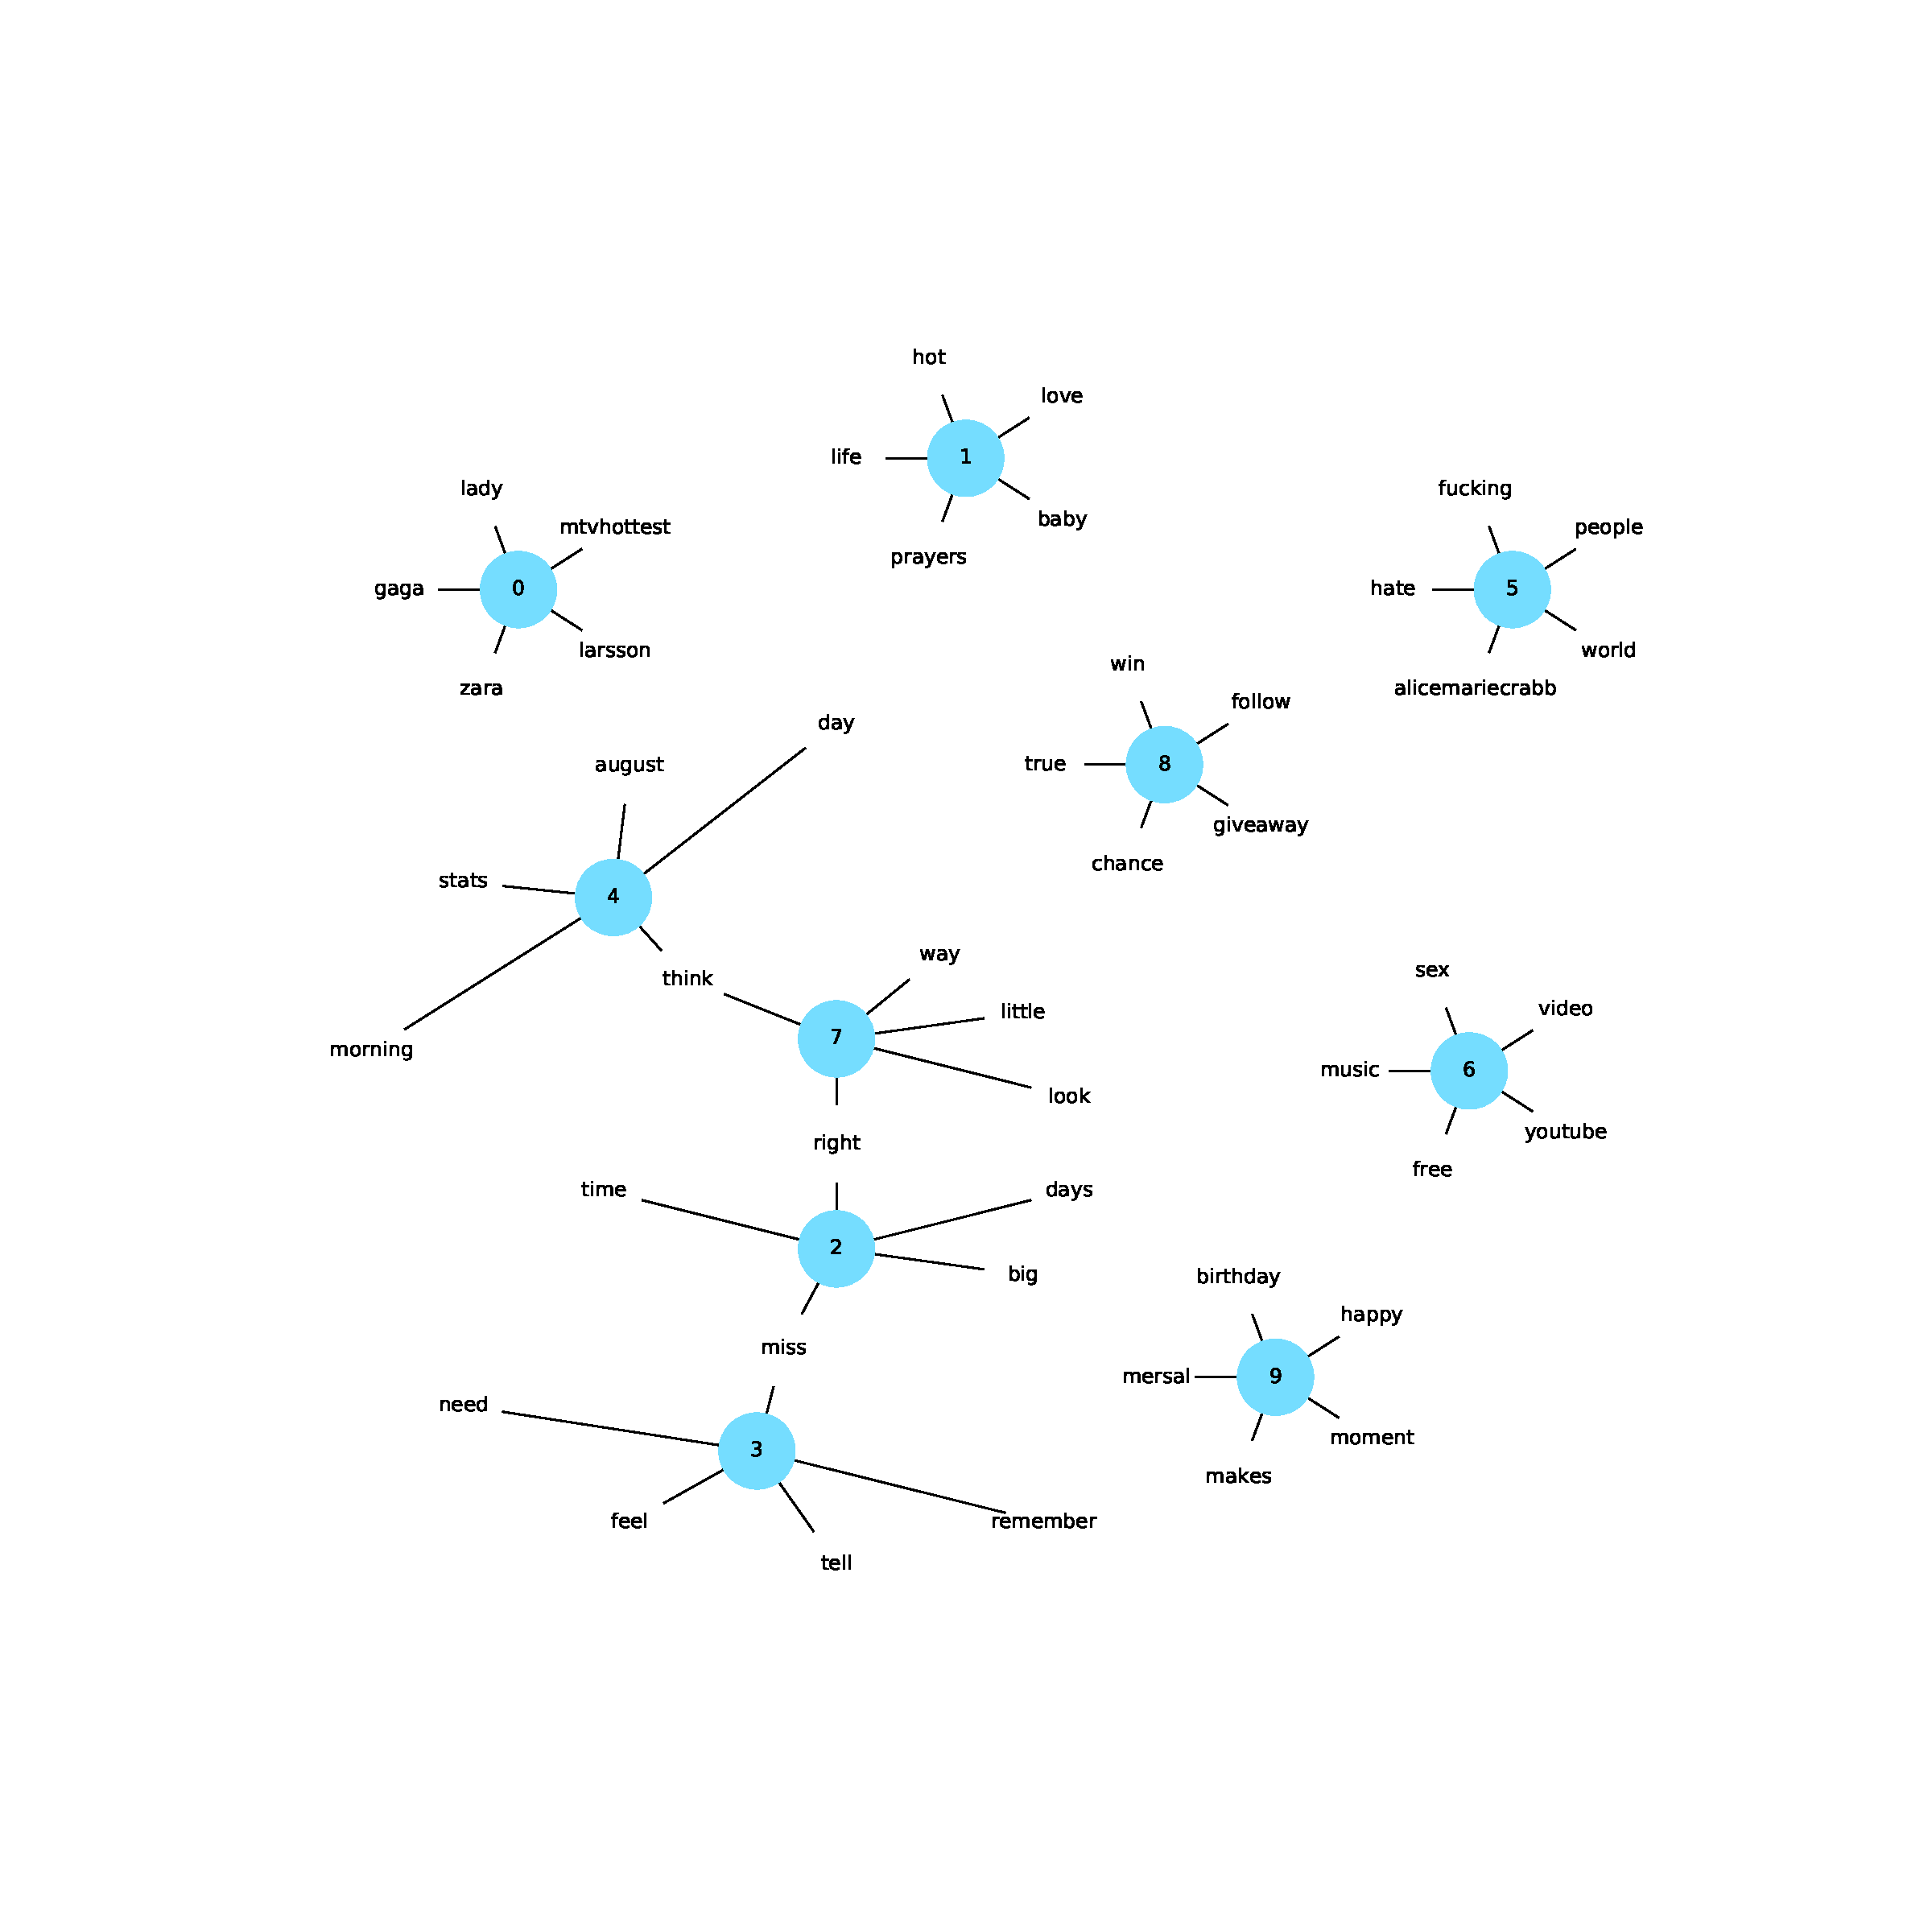
\includegraphics[width=\textwidth]{../figures/nmf_network_graph.pdf}
\end{figure}

\section{Results}
\label{sec:results}

Overall, the results that could be achieved with both methods were similar in terms of subjective descriptiveness of the top terms and amount of overlap.
There were even some equal topics, like topic number 6 in the LDA model and topic number 1 in the NMF model.
The advantages of NMF also do not apply to this usecase, therefore a decision was made in favor or LDA,
since it is the more mature method with more available research, implementations and tools like LDAvis, which can be used to comfortably
tune and explore models.

% !TEX root = ../main.tex
\chapter{Combining Sentiment Analysis and Topic Modeling}
\label{ch:combiningSentimentAnalysisAndTopicModeling}

% TODO write about "Joint sentiment/topic model for sentiment analysis" here or in the related-work section

In this chapter, the best sentiment analysis model from~\ref{ch:sentimentAnalysis}, naive Bayes,
is combined with the topic model built in~\ref{ch:topicModeling}, an LDA topic model,
to perform the sentiment analysis by topic model referred to in~\ref{ch:backgroundTheory}.
\\
This is achieved by simply performing the sentiment analysis on a Twitter status and attributing the result to each topic,
weighed by the percentage the status belongs to that topic given by the topic model.
A pseudo-code implementation of that can be seen in~\ref{pseudo_code:sentiment_topic_summing}.

\begin{figure}
    \caption{Summing up sentiments by topic for each status.}
    \label{pseudo_code:sentiment_topic_summing}
    % @formatter:off
    \begin{algorithmic}
        \State $topic\_sentiments \gets {}$ % TODO make sure that {} is the right way to init an object in pseudocode
        \For{$status$ in $statuses$}
            \State $topic\_probabilities \gets LDA(status)$
            \State $sentiment \gets naive_bayes(status)$
            \For{$topic,probability$ in $topic\_probabilities$}
                \State $topic\_sentiments[topic][sentiment] \gets topic\_sentiments[topic][sentiment] + probability$
            \EndFor
        \EndFor
    \end{algorithmic}
    % @formatter:on
\end{figure}

This results in a 2-dimensional array where all values sum up to the number of statuses,
since for each status the topic-probabilites sum up to 1.
A table showing the results for each topic with relative as well as absolute values can be seen in~\ref{tab:combination}.
The table also shows the sum of all probabilities, and the percentage of statuses in that topic.

\begin{table}
    \caption{Absolute and relative results of the sentiment-by-topic analysis.}
    \label{tab:combination}
    %\resizebox{\textwidth}{!}{%
    \begin{tabular}{l l l l l l l l l l l l} %
        \toprule
        & &
        \multicolumn{2}{c}{Positive}&
        \multicolumn{2}{c}{Neutral}&
        \multicolumn{2}{c}{Negative}&
        \multicolumn{2}{c}{Irrelevant}&
        \multicolumn{2}{c}{Sum}
        \\\cmidrule{3-12}
        Topic & Top 5 Terms
        & \%
        & Abs.
        & \%
        & Abs.
        & \%
        & Abs.
        & \%
        & Abs.
        & \%
        & Abs.
        \\\midrule
        0 & read, seo, old, board, actually & 64.40 & 11.14\% & 267.00 & 46.18\% & 56.67 & 9.80\% & 190.16 & 32.89\% & 578.23 & 9.00\% \\\midrule
        1 & time, single, playing, weekend, face & 74.44 & 11.43\% & 313.13 & 48.09\% & 92.87 & 14.26\% & 170.75 & 26.22\% & 651.19 & 10.14\% \\\midrule
        2 & need, give, damn, remember, already & 59.00 & 9.24\% & 302.46 & 47.39\% & 80.35 & 12.59\% & 196.43 & 30.78\% & 638.24 & 9.94\% \\\midrule
        3 & people, back, prove, sorry, tonight & 96.24 & 13.93\% & 320.69 & 46.40\% & 78.08 & 11.30\% & 196.10 & 28.37\% & 691.11 & 10.76\% \\\midrule
        4 & trump, enough, world, love, adamu & 69.94 & 11.08\% & 326.17 & 51.65\% & 79.75 & 12.63\% & 155.64 & 24.65\% & 631.50 & 9.83\% \\\midrule
        5 & home, people, morning, appears, shit & 82.30 & 12.48\% & 278.07 & 42.16\% & 94.26 & 14.29\% & 204.97 & 31.08\% & 659.59 & 10.27\% \\\midrule
        6 & love, win, chance, follow, enter & 63.83 & 10.96\% & 297.55 & 51.08\% & 53.85 & 9.24\% & 167.27 & 28.72\% & 582.51 & 9.07\% \\\midrule
        7 & mtvhottest, lady, gaga, larsson, zara & 42.43 & 7.65\% & 253.08 & 45.62\% & 43.23 & 7.79\% & 216.02 & 38.94\% & 554.75 & 8.64\% \\\midrule
        8 & miss, sexy, sex, naked, outfit & 79.47 & 11.54\% & 344.14 & 49.97\% & 63.95 & 9.29\% & 201.15 & 29.21\% & 688.71 & 10.72\% \\\midrule
        9 & tell, someone, feel, every, preaching & 74.32 & 10.80\% & 327.11 & 47.54\% & 94.52 & 13.74\% & 192.12 & 27.92\% & 688.05 & 10.71\% \\\midrule
        \\\bottomrule
    \end{tabular}
\end{table}

To visualize the sentiment by topic,
the network graph used in~\ref{ch:topicModeling} was extended.
The size of a node representing a topic indicates the topics' prevalence in the dataset.
The color, on a hue-spectrum from red to green, represents the polarity.
% TODO  seen in \ref{fig:hue_spectrum},
On a 360\degree hue-spectrum in the HSV-color-space, 0\degree is red, and 120\degree is green.
The opacity is determined by the subjectivity.
The exact formulae can be seen in~\ref{math:visualization}.


\begin{figure}
    \caption{Definition of precision, recall and F-measure~\cite{Hong2010}.}
    \label{math:visualization}
    \begin{align*}
        % TODO proper variable names, introduced at the beginning, i.e. p = sum of "positive" probabilites for topic
        size = positive + negative + neutral + irrelevant
        hue = positive / (positive + negative)
        opacity = (positive + negative) / (positive + negative + neutral)
        size = percentage of statuses in that topic \* 2000 && Size between 0 and 2000
    \end{align*}
\end{figure}

To make these values visually more differentiable, they were then scaled.
Hue was linearly scaled s.t. the smallest value was 0\degree (red) and the biggest value was 120\degree (green).
The saturation was linearly scaled s.t. the smallest opacity was 0\%,
and the biggest opacity was 80\%.
20\% were then added to each node so that each node would be visible.
The size was linearly scaled to be between 0 and 2000.
The resulting network graph can be seen in~\ref{fig:combined_network_graph}.

\begin{figure}
    \centering
    \caption{Network graph of the LDA topic model created from the stream sample dataset}
    \label{fig:combined_network_graph}
    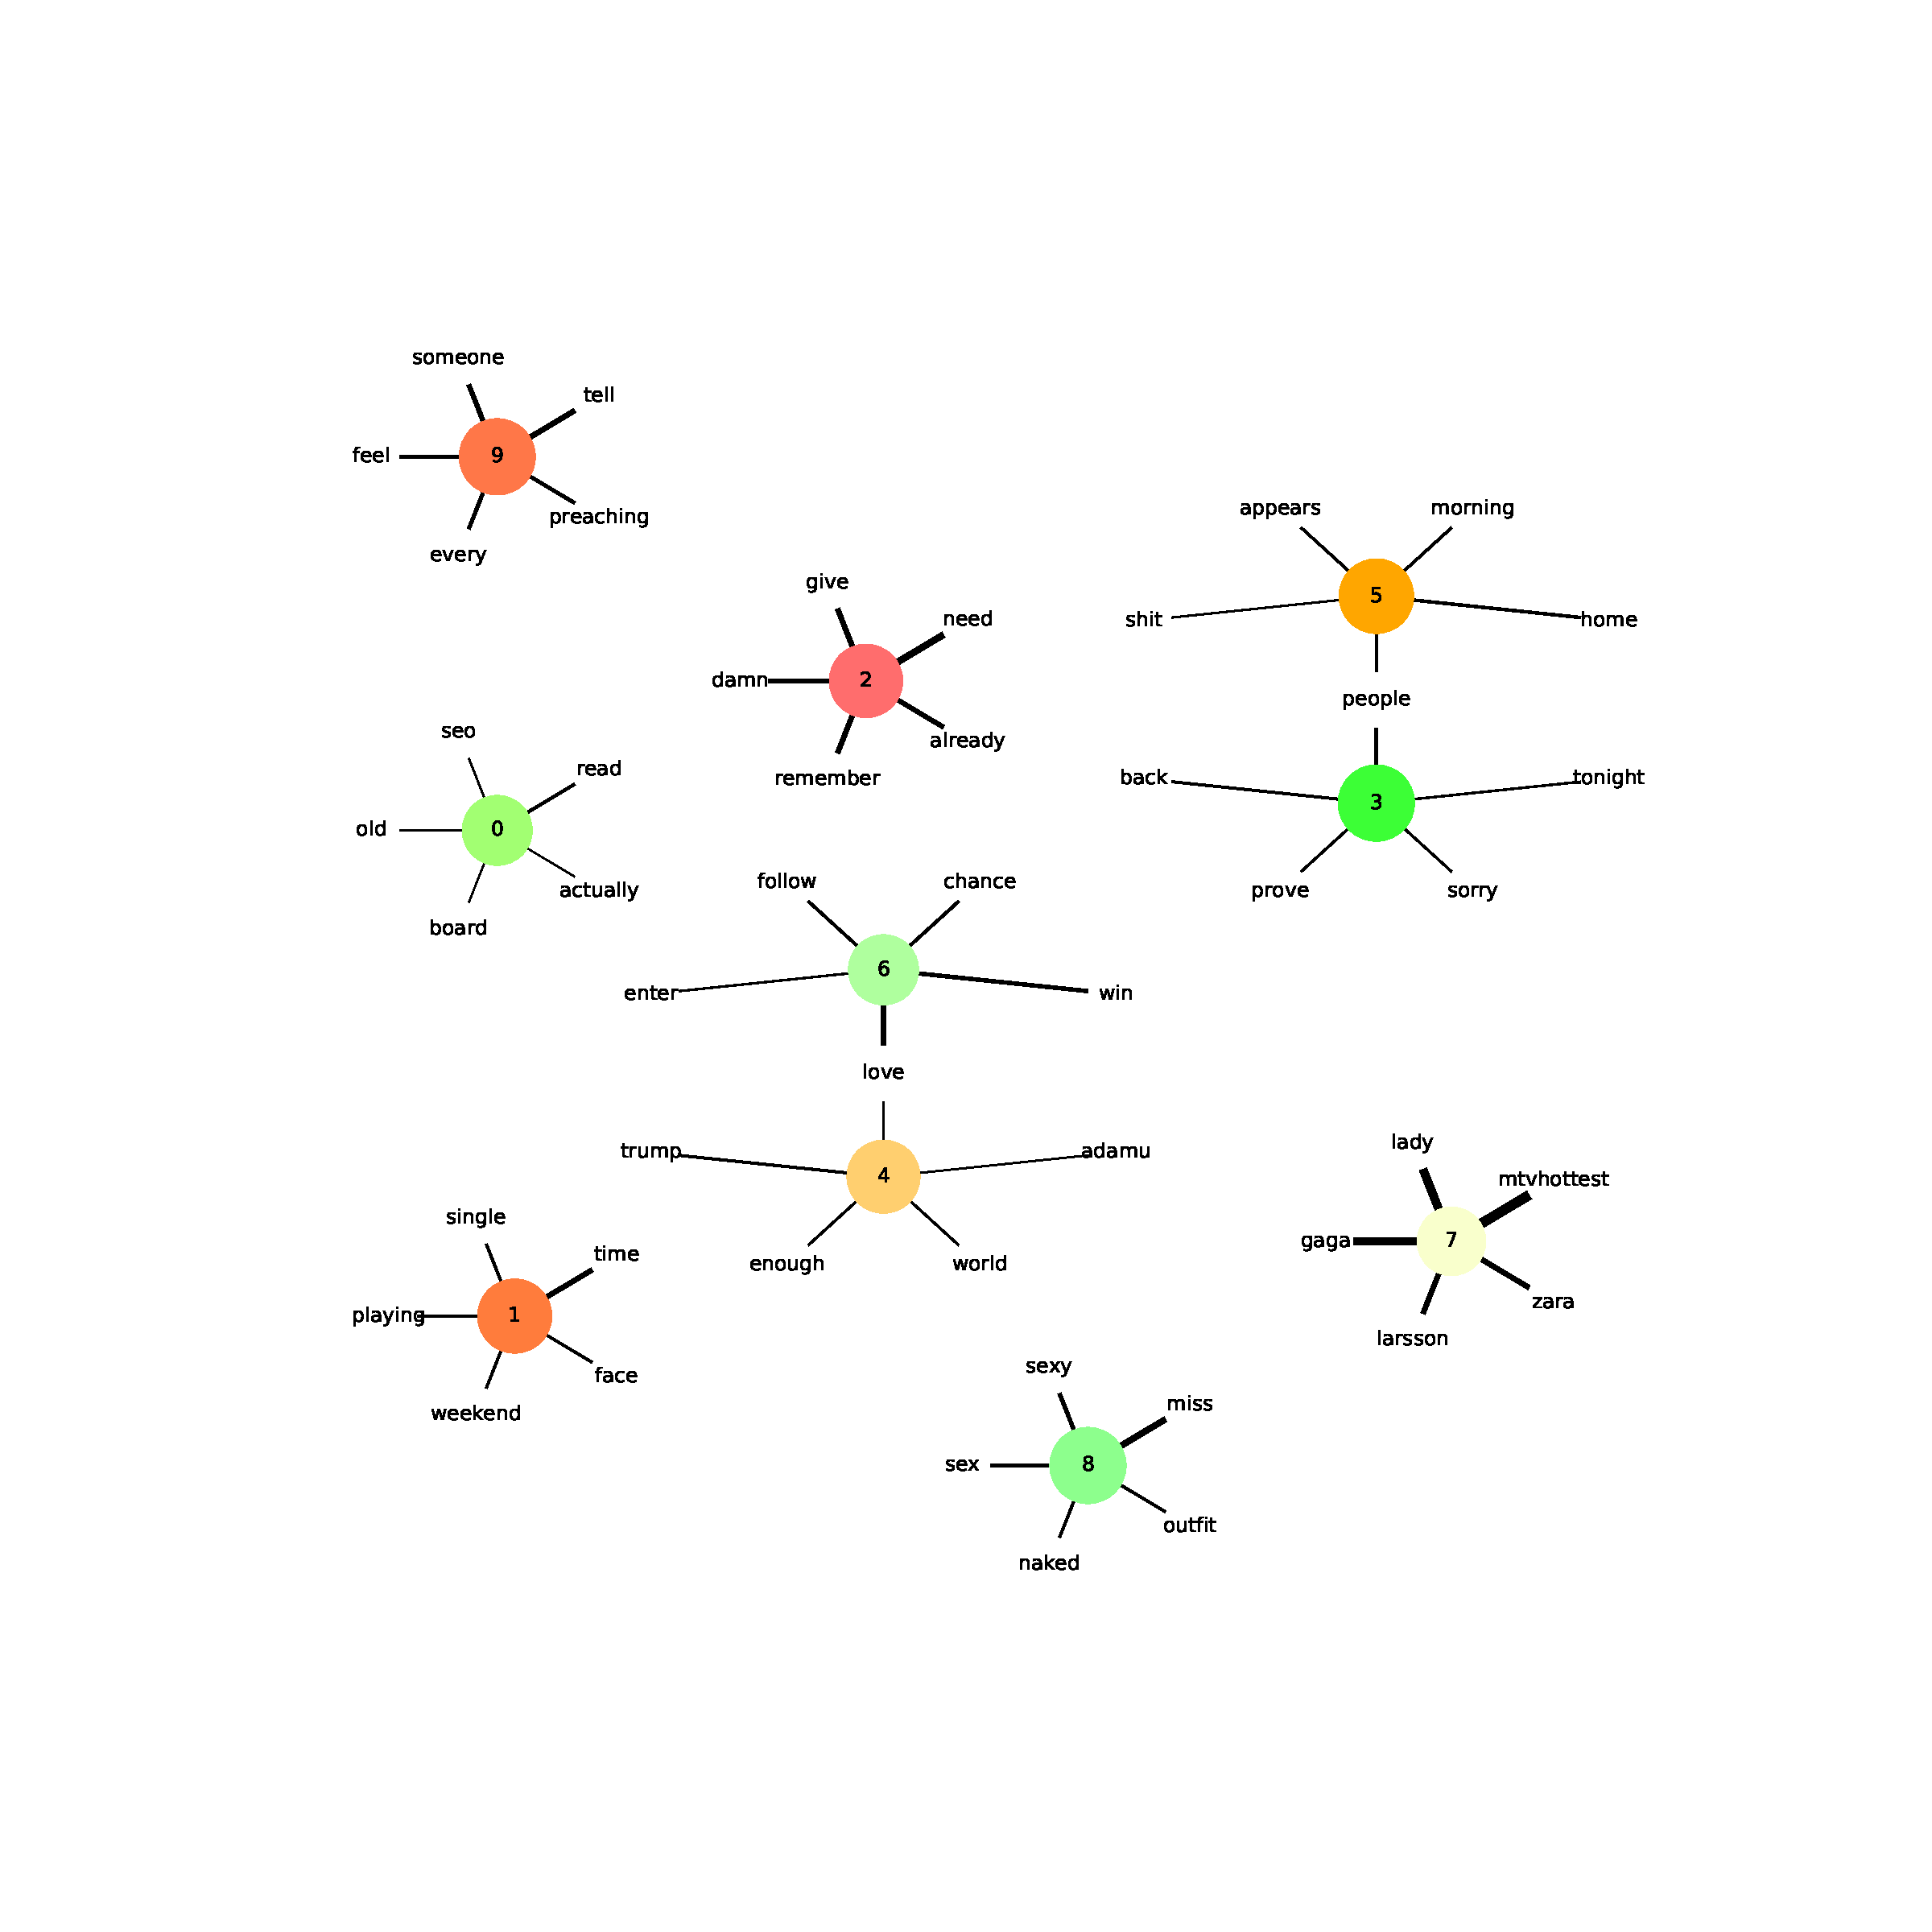
\includegraphics[width=\textwidth]{../figures/combined_network_graph.pdf}
\end{figure}
% !TEX root = ../main.tex
\chapter{Dashboard}
\label{ch:dashboard}

Since the one of the goals of this thesis was to make these analyses available to a broader,
semi-technical audience, as described in~\ref{ch:goals},
a user-friendly streaming dashboard was created.
\\
This dashboard puts all the aforementioned theory into practice,
using the Twitter streaming API instead of data at rest,
as described in~\ref{subsec:dataAtRest-DataInMotion},
making it one of the most important chapters.

\section{Requirements}
\label{sec:requirement}

To make it easily accessible, it was decided to implement the dashboard as a web-based application.
Since it has to perform the analyses on streamed data from Twitter,
and the streaming API is rate limit as described in~\ref{subsec:streaming},
each user needs to authenticate with a Twitter account.
That way, the application can scale with the number of users,
without the number of connection requests being limited by the application-rate-limit.
\\
A settings-dialog is required to enable the user to choose between any of the streams explained in~\ref{subsec:streaming},
and to configure all their respective parameters.
\\
To give the user a feeling for the stream he/she configured,
the 100 most recently streamed statuses are listed in a feed.
\\
Since the dashboard will not allow the user to train new models,
the best model for sentiment analysis, developed in~\ref{ch:sentimentAnalysis},
the best model for topic modeling, developed in~\ref{ch:topicModeling},
and the combination of both, developed in~\ref{ch:combiningSentimentAnalysisAndTopicModeling}
should be used to classify incoming statuses.
\\
The results of this classification should be visualized over time,
necessitating visualizations different to the previously used scatter plots, network graphs and pie charts.

\section{Architecture}
\label{sec:architecture}

The architecture of the dashboard is a simple client-server architecture.
To facilitate the analyses of the Twitter stream,
Kafka was used as a distributed messaging system as described in~\ref{subsec:kafka},
and Spark was used for distributed processing of the messages, as described in~\ref{subsec:spark}.
A simplified diagram of the architecture can be seen in~\ref{fig:architecture}.

\begin{figure}
    \centering
    \caption{Simplified diagram of the architecture}
    \label{fig:architecture}
    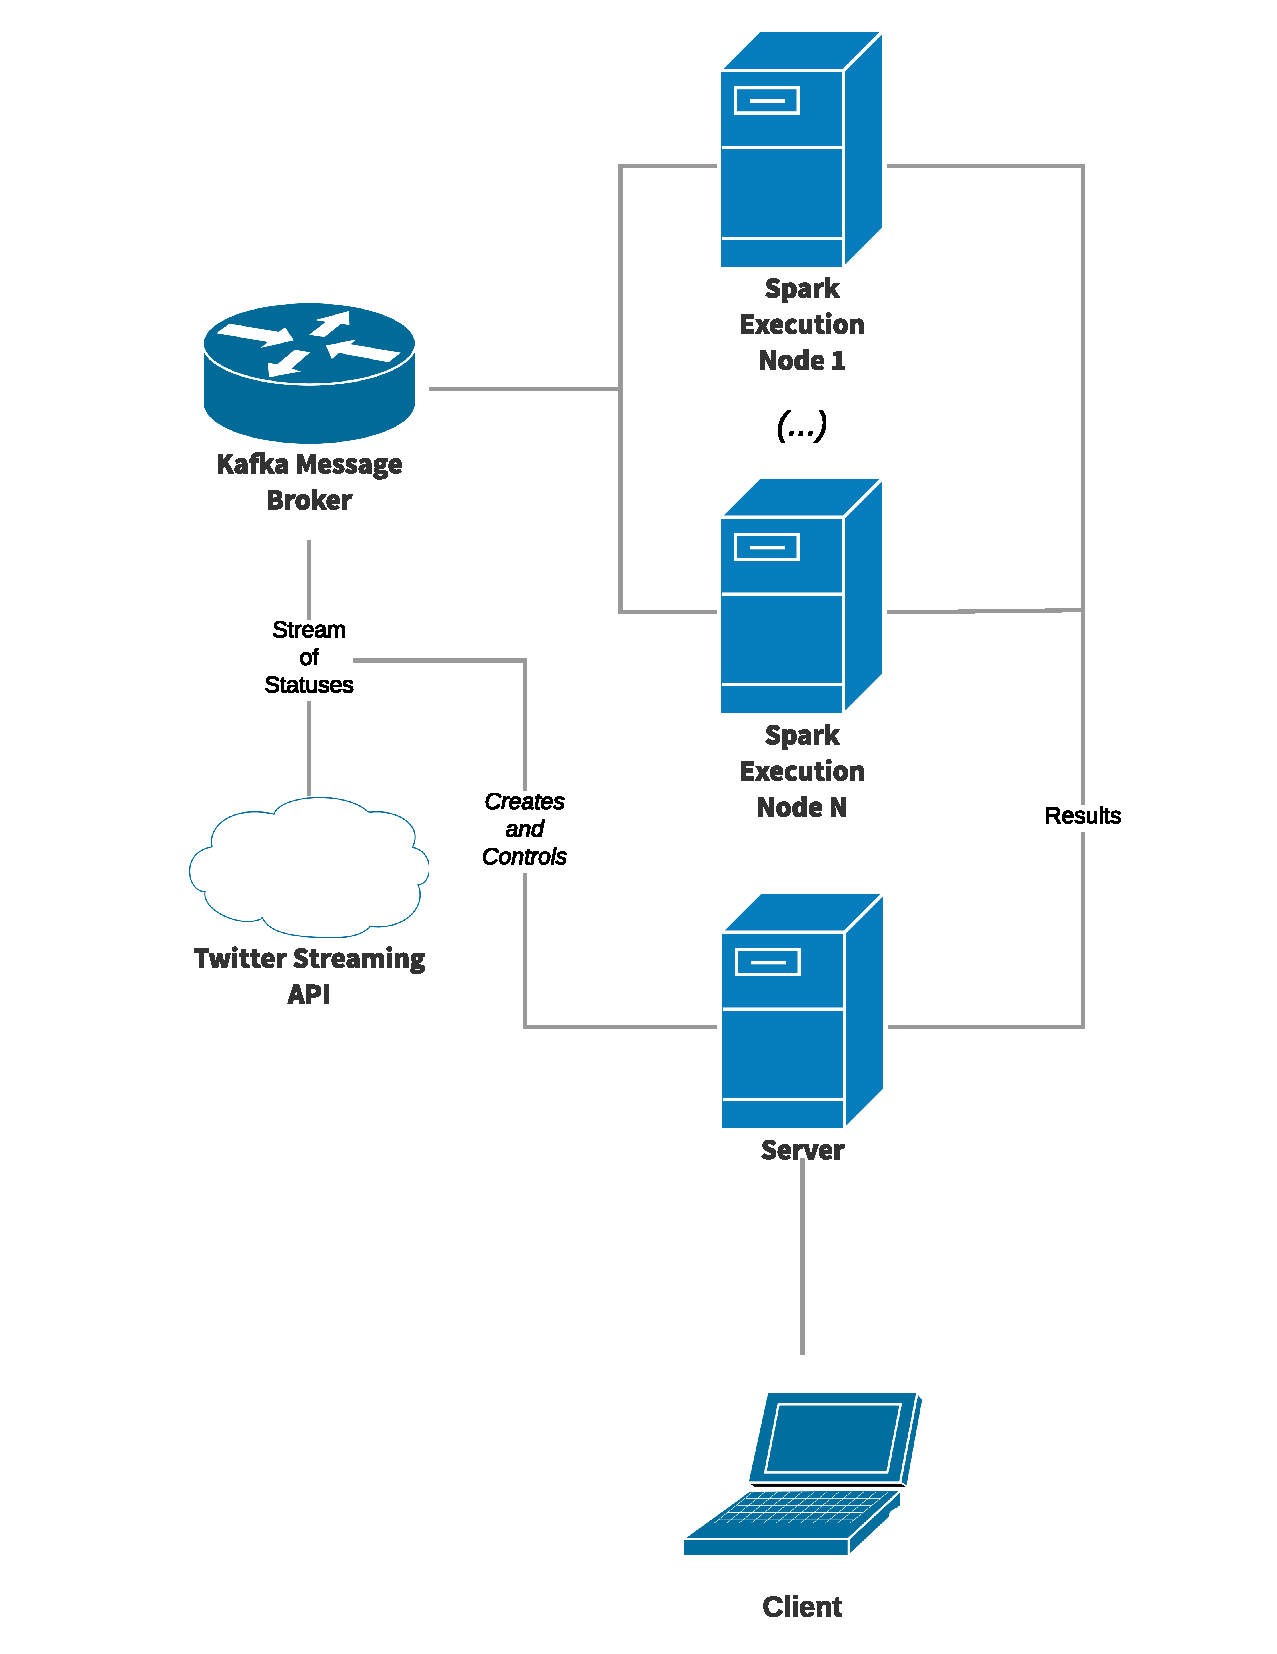
\includegraphics[width=10cm]{../figures/architecture.pdf}
\end{figure}

For the server, Flask~\cite{flaskDocs} was used, because it is written in Python and therefore works seamlessly with the rest of the code.
In the frontend, common web technologies such as HTML, CSS and JS were used, with Angular JS providing the framework~\cite{angularDocs}.
Furthermore, some miscellaneous technologies such as SCSS\cite{scssDocs} for more efficient styling and the taskrunner GruntJS~\cite{gruntDocs} for
minification, transpilation etc. were used.

\section{Dashboard Code Structure}
\label{sec:dashboardCodeStructure}

The dashboard application is located under \texttt{Thesis/src/visualization} in the structure of the whole thesis explained
in~\ref{forest:dscookiecutter}.
This directory does not contain the code used for creating and analyzing the stream,
which, as described in~\ref{sec:projectStructure}, is located under \texttt{Thesis/streaming}.
On the first level, the structure is type-based, separating between client- and server-related code.
Since the type of asset (python-scripts for the server-related code, HTML/CSS/Javascript for the client-related code)
remains constant on every level below that, the structure is then switched to component-based.
With this structure, full advantage can be taken of the modular nature of AngularJS~\cite{angularDocs}.
% TODO search for Javascript to make casing/hyphenation consistent
The structure of the dashboard-application part of the project can be seen in~\ref{forest:dashboard}.

% TODO use the folder icon in all forest https://tex.stackexchange.com/questions/5073/making-a-simple-directory-tree
\begin{figure}
    \caption{Structure of the dashboard-application part of the project under \texttt{Thesis/src/visualization}}
    \label{forest:dashboard}
    \begin{forest}
        % @formatter:off
% TODO can this be safely indented? same as code
  for tree={
    font=\ttfamily,
    grow'=0,
    child anchor=west,
    parent anchor=south,
    anchor=west,
    calign=first,
    edge path={
      \noexpand\path [draw, \forestoption{edge}]
      (!u.south west) +(7.5pt,0) |- node[fill,inner sep=1.25pt] {} (.child anchor)\forestoption{edge label};
    },
    before typesetting nodes={
      if n=1
        {insert before={[,phantom]}}
        {}
    },
    fit=band,
    before computing xy={l=15pt},
  }
[visualization
  [dashboard \textit{contains client and server code for the dashboard application}
    [client
      [main \textit{The main (home) page}
      ]
      [main \textit{The actual dashboard}
      ]
    ]
    [server
      [api \textit{Facilitates interaction between the frontend and the stream}
      ]
      [auth \textit{All functionality for the authentication with Twitter}
      ]
    ]
  ]
]
        % @formatter:on
    \end{forest}
\end{figure}

\section{Implementation and Testing}
\label{sec:implementation}

%TODO put some vital code pieces in the appendix

Updating the settings was implemented as a HTML-form, styled with Bootstrap~\cite{bootstrapDocs},
and allows selecting which stream to analyze and modifying all its parameters as per the documentation~\cite{twitterDocs},
also explained in~\cite{subsec:streaming}.
A screenshot of the settings dialog of the dashboard can be seen in~\ref{fig:dashboard-settings}.

\begin{figure}
    \centering
    \caption{The settings dialog of the dashboard}
    \label{fig:dashboard-settings}
    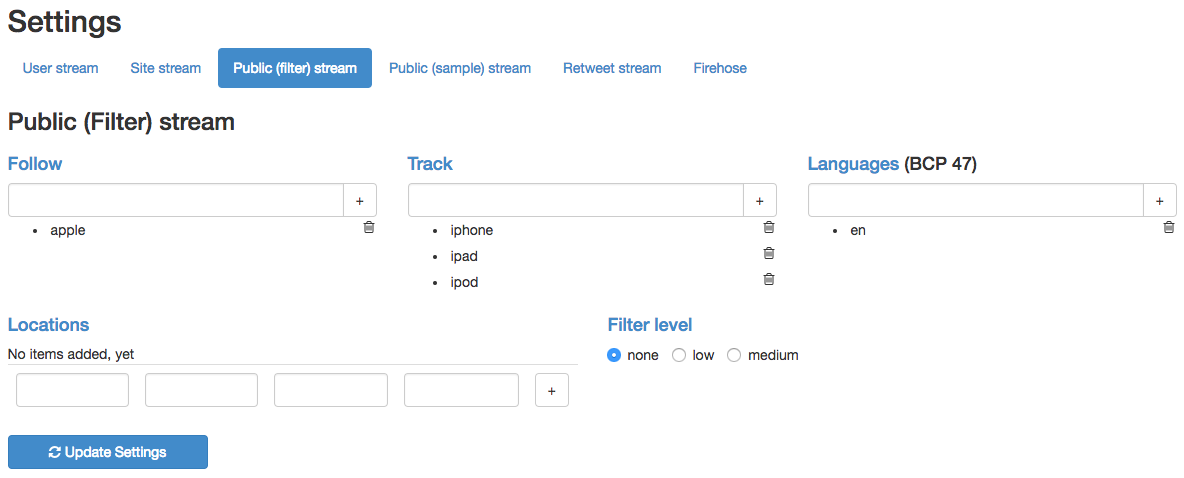
\includegraphics[width=10cm]{../images/dashboard_settings.png}
\end{figure}

When clicking the update-button, the current settings are sent to the server via a websocket,
which then closes the existing stream (if any), and opens a stream with the new settings.
\par
Incoming statuses are relayed into the Kafka messaging system described in~\ref{subsec:kafka}.
Kafka then distributes the statuses to the Spark execution nodes as described in~\ref{subsec:spark}.
\\
Preprocessing, tokenization, analyses and classifications was combined into one sparkjob.
This saves bandwidth, as some data like the dictionary might otherwise be transmitted to the execution nodes twice,
since both sentiment analysis and topic modeling use it.
Also, this way, each status only needs to go through one execution node,
and the computational power required per status is still small enough for Kafka to distribute them efficiently.
Furthermore, this makes it easier to combine the results of sentiment analysis and topic modeling later on.
However, as explained in~\ref{subsec:nltk}, the NLTK is meant for teaching and research,
and the naive bayes classifier built with it did not meet the performance demands in a streaming scenario,
so an exact replica of the classifier was built using scikit~\cite{scikitDocs}, and used instead.
The resulting function, applied on the incoming statuses on the execuption nodes, can be seen in~\ref{fig:spark_job}

\begin{figure}
    \caption{Example usage of the NLTK in a Python shell}
    \label{code:nltk}
    % @formatter:off
    \begin{minted}{python}
    def analyze(element):
        # The actual tweet is the second element in a tupel
        tweet_str = element[1]
        # It's still a string, so parse it
        tweet = json.loads(tweet_str)
        # Just the text needed
        raw_text = tweet['text']
        # Using the same preprocessing function as everywhere else, for consistency
        text = preprocess(raw_text)
        # Use the same tokenization functions as everywhere else, for consistency...
        # ...without stopword removal for sentiment classification
        tokens_sa = sa_tokenize(text)
        # ... with stopword removal for topic modeling
        tokens_lda = lda_tokenize(text)

        # The update should contain...
        update = dict()
        # ...the sentiment...
        update['sentiment'] = analyze_sentiment(tokens_sa)
        # ...the topics...
        update['topics'] = model_topics(tokens_lda)
        # ...and the tweet itself (or at least what we need from it in the frontend).
        update['tweet'] = {
            'text': raw_text,
            'user': {
                'name': tweet['user']['name']
            }
        }

        return update
    \end{minted}
    % @formatter:on
\end{figure}

The update containing the results and the tweet itself is then sent to the master node,
which is also the server as seen in~\ref{fig:architecture},
and sent to the client via a websocket.
\par
The client keeps a FIFO-queue of all incoming updates, facilitating a sliding window of the analysed statuses.
This way, a moving average can be calculated on the values, which represents the overall, \textit{average},
sentiment and topics on Twitter, without too much delay.
The size of this queue, or \textit{window size}, has to be chosen carefully to reduce noise without suppressing actual signals.
A good window size was found to be \texttt{200}.
As described in~\ref{sec:requirement}, the visualizations needed to be changed to incorporate a time-line.
To visualize changes in the incoming tweets in real time, the results were plotted in a continually moving line chart over time.
The library Smoothie Chart~\cite{smoothieDocs} was used to implement these charts.
For all of these charts, one vertical gridline represents one second.
\par % testing TODO maybe subsection
For testing, the filter stream was used,
the language was set to english (since our models are trained on english data only),
and only one keyword was tracked.
% First test: sentiment TODO again, these should be sub
First, the keyword was set to\texttt{iPhone},
and the stream was left running until the queue was filled and all results calculated from fewer elements
(which might look noisy) were no longer visible on the time-line. % TODO is timeline not a word? Make consistent!
Then, to artificially provoke a change in sentiment,
the streaming settings were updated to only track the keyword \texttt{people} without resetting the charts or the queue (and therefore the moving average).
This illustrates what a sudden change in sentiment for a stream would look like if it were observed naturally.
The resulting graph, and the associated values, can be seen in~\ref{fig:dashboard-sentiment}

\begin{figure}
    \centering
    \caption{The sentiment chart plus values, showing the change in sentiment after changing the stream settings}
    \label{fig:dashboard-sentiment}
    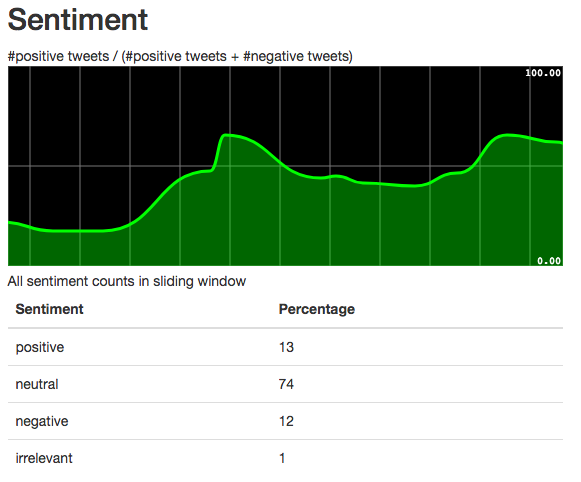
\includegraphics[width=10cm]{../images/dashboard_sentiment.png}
\end{figure}

% Second test
4 and 9, at the cost of 5
After running the stream with these settings for a while, a natural change in topics was observed, which can be seen in~\ref{fig:dashboard-topics}.
Even though the keyword was still \texttt{people}, and the dominating topic was, obviously, topic number 5,
for which this keyword is one of the most likely ones, the prevalence of this topic decreased in favor of topics 4 and 9,
indicating a wave of tweets associated with these topics occurring at that moment.
These events could be observed regularly, and might even indicate bot activity~\cite{chu2012detecting}.

\begin{figure}
    \centering
    \caption{The topics chart plus values, showing the naturally occuring change in topic distribution}
    \label{fig:dashboard-topics}
    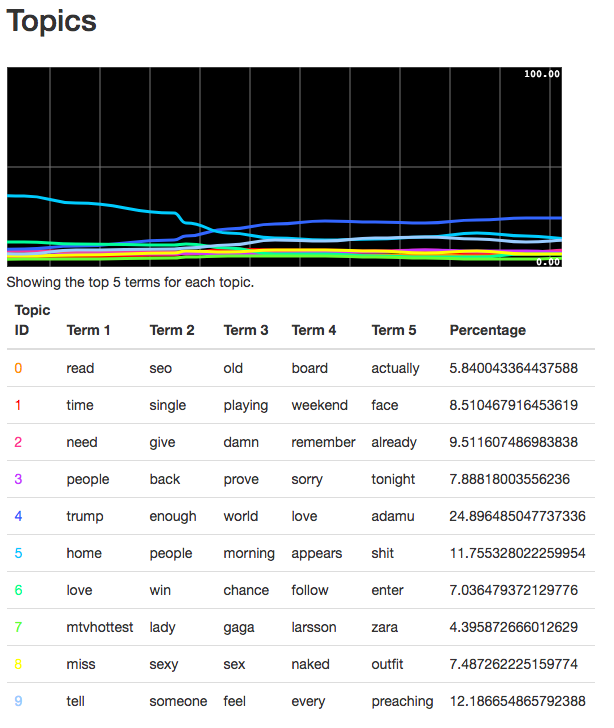
\includegraphics[width=10cm]{../images/dashboard_topics.png}
\end{figure}

% Third test

To calculate the sentiment by topic for the combination-visualization,
the sliding window was set to 1000, since topics with little prevalence and few opinionated statuses
(those that are labeled positive or negative) would give very noisy results otherwise.
That window size was found to give the right balance between reducing noise and not suppressing any signal.
\par
Even though the sentiments by topic were mostly free of noise, they did not converge,
indicating that some topics have an inherently different sentiment.
\par
As with the visualization of sentiment, % TODO reference here if that becomes a subsection
the settings were changed from tracking \texttt{apple} to tracking \texttt{weekend}, to illustrate a change in sentiment by topic.
This still gave interesting results, however, showing that depending on which keywords the stream is parameterized with,
the sentiment per topic differs.
The resulting graph and associated values can be seen in~\ref{fig:dashboard-sentiment-by-topic}.

\begin{figure}
    \centering
    \caption{The sentiment by topic chart plus values, showing the change in sentiment by topic after changing the stream settings}
    \label{fig:dashboard-sentiment-by-topic}
    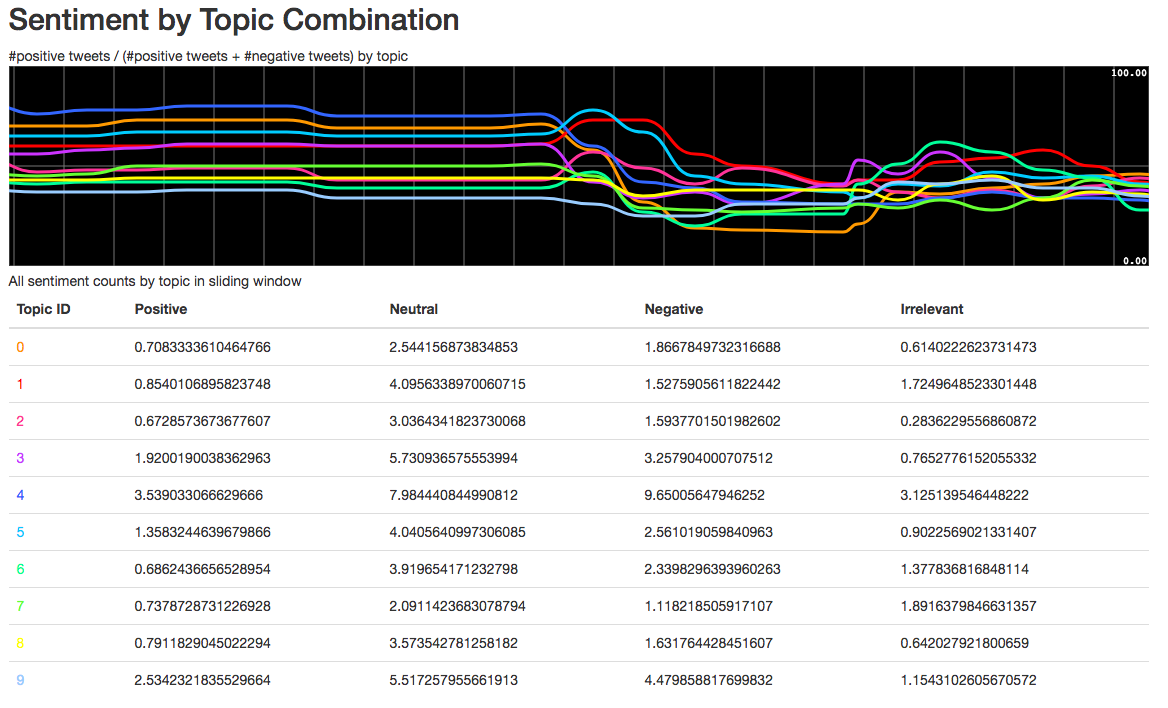
\includegraphics[width=10cm]{../images/dashboard_sentiment_by_topic.png}
\end{figure}

\par
The part of the dashboard showing actual statuses coming in to give the user a feeling for the stream is not shown here due to Twitter's TOS.


%% ---------------------------------------------------------------------------
%%
%% Results and Conclusion
%%
%% ---------------------------------------------------------------------------
\part[Results and Conclusion]{Results and Conclusion}
\label{part:resultsAndConclusion}
% !TEX root = ../main.tex
\chapter{Results}
\label{ch:results}

When streaming from the sample stream, from which the sample dataset was collected,
the topic distribution does not approach that of the sample dataset.
While the topic distribution on the training dataset is close to equally distributed as seen in~\cref{fig:sample_topic_distribution},
the same cannot be said for the topic distribution on the same stream on September $27^{th}$ 2017, more than two months later,
as seen in~\cref{fig:sample_topic_distribtion_new}.

\begin{figure}
    \centering
    \caption{Topic distribution of new data, with the LDA model trained on the sample dataset}
    \label{fig:sample_topic_distribtion_new}
    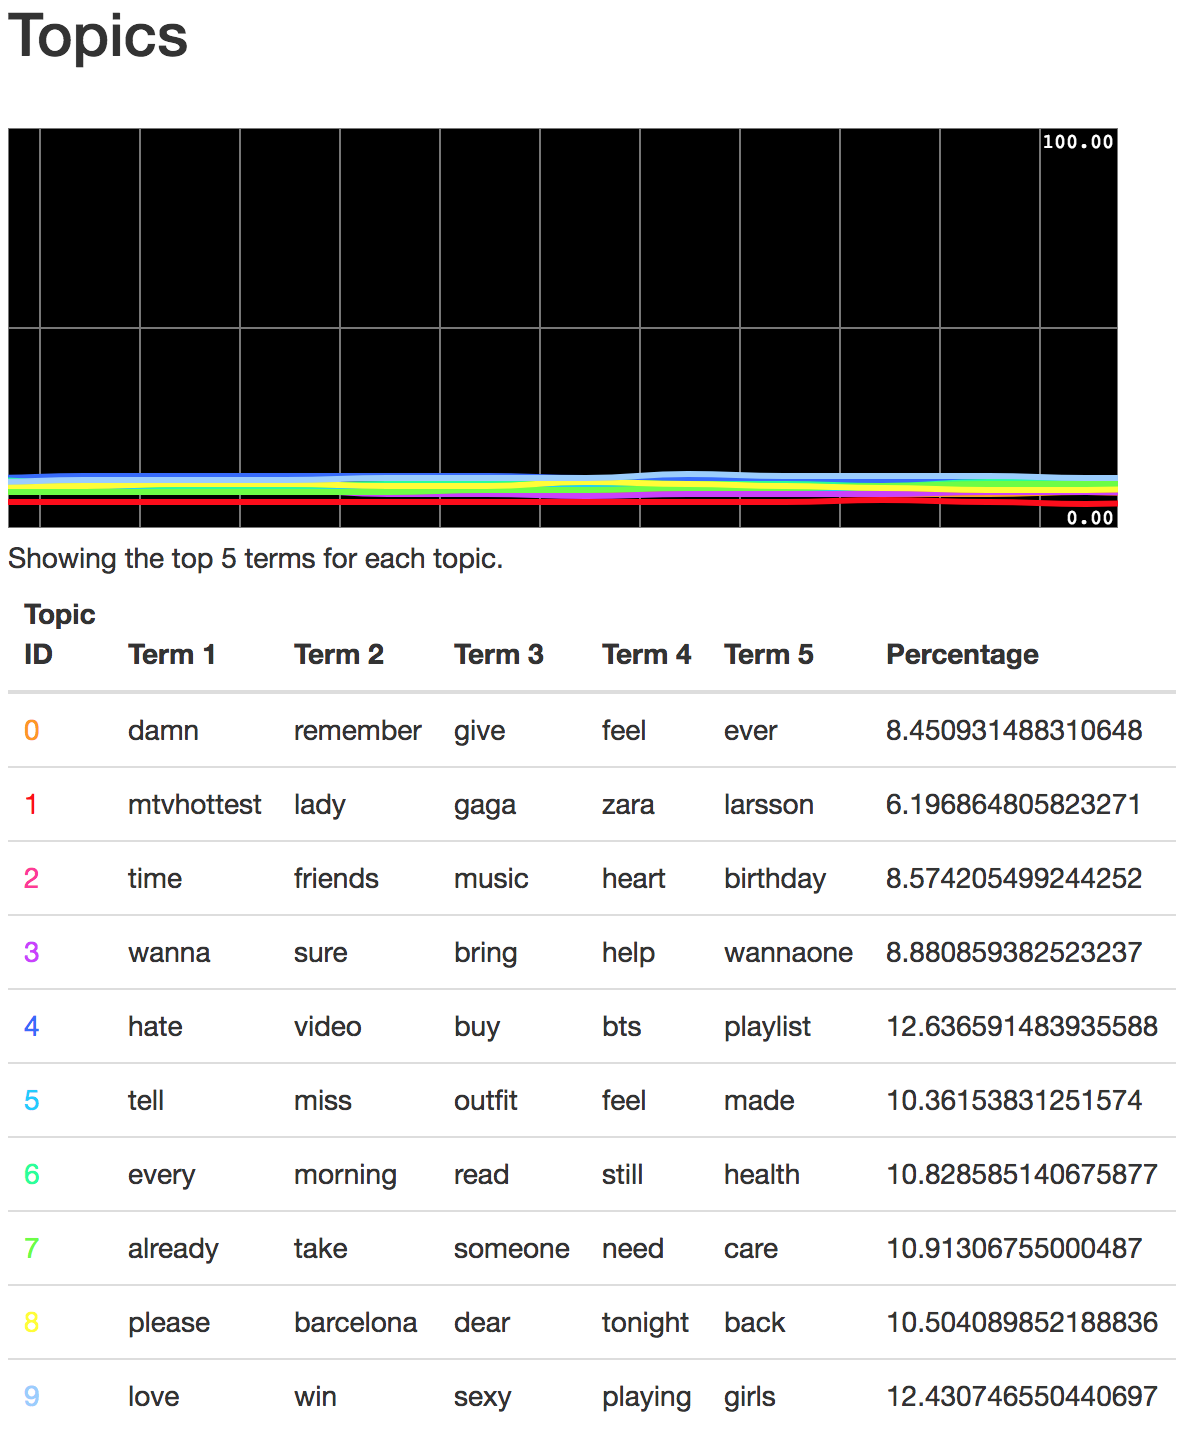
\includegraphics[width=\textwidth]{../images/dashboard_topics_sample.png}
\end{figure}

This time, topics with top terms that indicate some event, like "mtvhottest", are lower in prevalence,
in favor of topics with more general terms.\\
This indicates that while the dashboard can reliably show changes in what users are talking about on Twitter,
as demonstrated in~\cref{sec:testing},
it might not be able to accurately model new, emerging topics.
For this reason, it also does not make sense to compare the sentiment by topic distributions,
since the meaning of topics changed.

The same comparison was however made for sentiment analysis, comparing the sentiment distribution in the sample dataset, seen in~\cref{fig:sample_sentiment},
to the sentiment distribution observed through the dashboard on the 27$^th$ of September 2017, seen in~\cref{fig:sample_sentiment_distribtion_new}.

\begin{figure}
    \centering
    \caption{Sentiment distribution of new data, with the naive bayes model trained on the Sanders dataset}
    \label{fig:sample_sentiment_distribtion_new}
    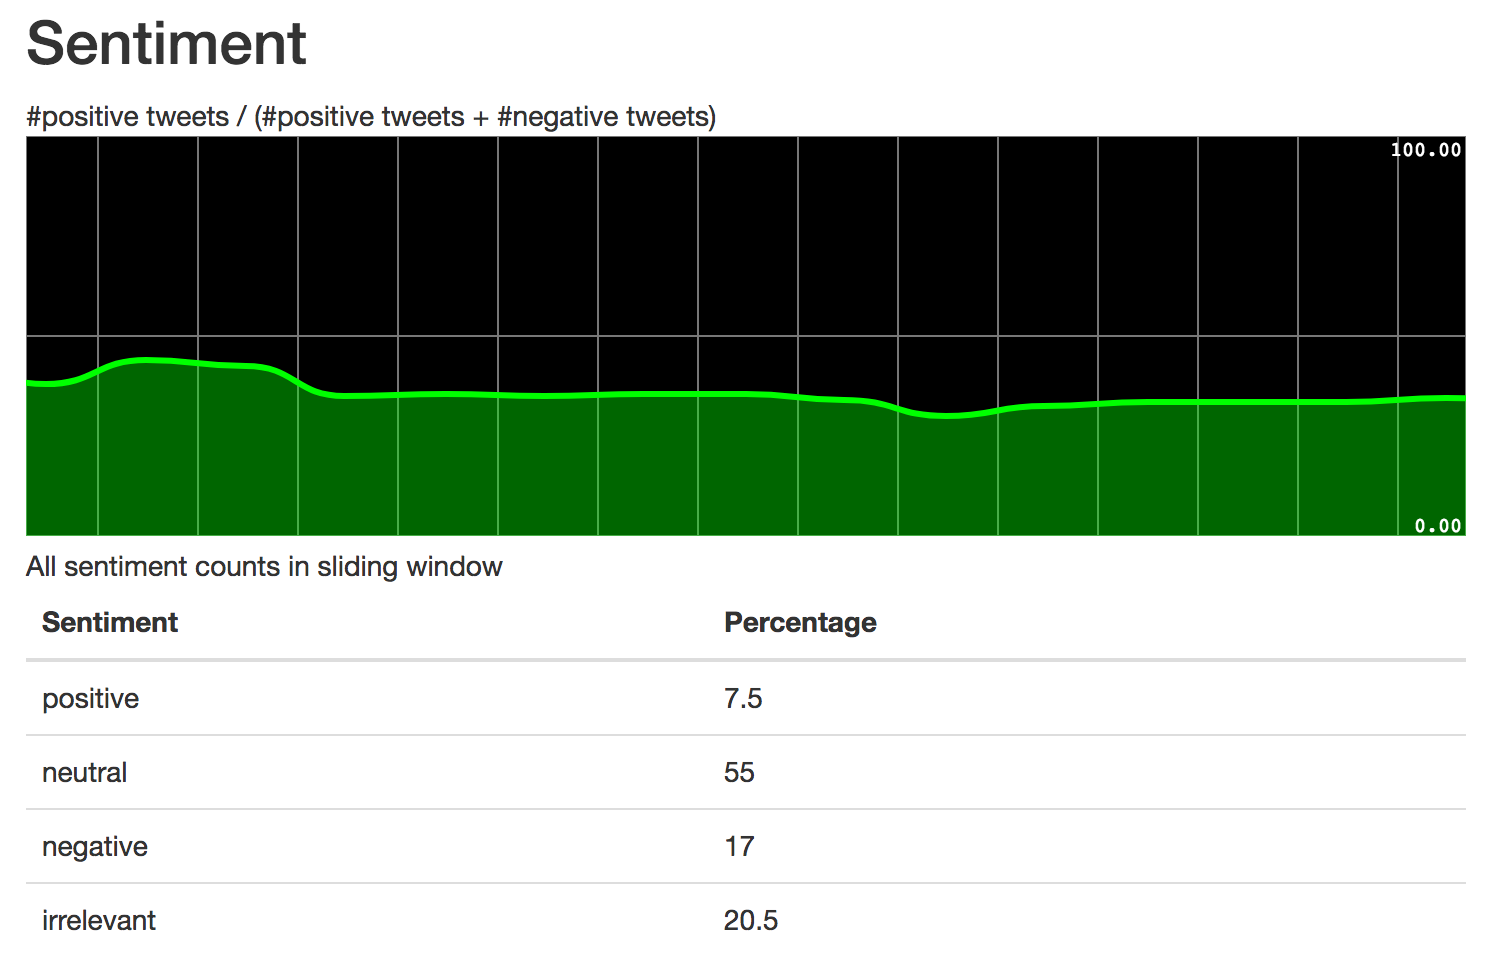
\includegraphics[width=\textwidth]{../images/dashboard_sentiment_sample.png}
\end{figure}

This comparison shows that the sentiment on the stream remained on a similar level than in the sample dataset,
and did not change as much as the topics did, indicating that while the topics twitter users post statuses about change,
the overall, average sentiment, remains relatively constant.

In spite of some shortcomings, the dashboard therefore still provides interesting insights and monitoring capabilities.\\
It can, for example, be used to track a companies Twitter feed during a critical event, using the user stream.
This would provide an objective indication of the events impact on customer sentiment,
and enable the company to react in real time without having to base a decision on few, manually observed interactions.\\
It can also be used to monitor a stream for sudden changes in topic,
indicating the occurrence of an event that might be of interest for the monitoring entity.
% !TEX root = ../main.tex
\chapter{Conclusion}
\label{ch:conclusion}

Hypothesize counteractions to impending shitstorms using real-time detection (is this the right chapter for that?).
Around 1 page.
\pagebreak[1]


% !TEX root = ../main.tex
\chapter{Open Source Contributions}
\label{ch:openSourceContributions}

Some open source contributions were made in the process implementing this thesis, they are listed here.
Where it made sense (low cohesion), parts of the projects were outsourced into packages etc. to be more manageable.

\begin{itemize}
    \item
    Pyspark lda streaming
    \item
    Quantitative comparison of Sentiment Analysis algorithms for twitter data
    \item
    Sanders dataset hydration script (sanders-fast-download), because the dataset is good but hard to come by
\end{itemize}

This should also be around 1 page long.
\pagebreak[1]
% !TEX root = ../main.tex
\chapter{Further Work}
\label{ch:furtherWork}

\begin{itemize}
    \item
    Contributions to the platform itself and associated open source stuff
    \item
    Using the platform, since it was designed to be usable for research of semi-technical researchers
    \item
    Using the evaluations made in other projects (e.g. twitter sentiment classification methods, charting library comparison)
    \item
    Research the impact of filtering out spam and bots, incorporating informativeness-measures into the evaluations

\end{itemize}


% ---------------------------------------------------------------------------
%
% Appendix
%
% ---------------------------------------------------------------------------
\part*{Appendix}
\addcontentsline{toc}{part}{Appendix}

\appendix %---------------------------------------

% !TEX root = ../main.tex
\chapter{Detailed Descriptions}
%\section{Detailed Validation Results}
\label{chapter:DetailedDescriptions}\label{appendix}
%\inputminted{c++}{../../src/wos_native.cuh}
\newpage



    \clearemptydoublepage

    \printglossaries

    \addcontentsline{toc}{chapter}{Bibliography}
    \bibliography{bibliography/literature}

\end{document}
